\documentclass[review]{elsarticle}

\usepackage{lineno,hyperref}
\modulolinenumbers[5]
%\usepackage[margin=2cm]{geometry}
\usepackage[justification=centering]{caption}
\usepackage{subfig}
\usepackage{multirow}
\usepackage{xcolor}
\usepackage{setspace}
\doublespacing
\renewcommand{\arraystretch}{1.1}
\journal{Pattern Recognition}

%%%%%%%%%%%%%%%%%%%%%%%
%% Elsevier bibliography styles
%%%%%%%%%%%%%%%%%%%%%%%
%% To change the style, put a % in front of the second line of the current style and
%% remove the % from the second line of the style you would like to use.
%%%%%%%%%%%%%%%%%%%%%%%

%% Numbered
%\bibliographystyle{model1-num-names}

%% Numbered without titles
%\bibliographystyle{model1a-num-names}

%% Harvard
%\bibliographystyle{model2-names.bst}\biboptions{authoryear}

%% Vancouver numbered
%\usepackage{numcompress}\bibliographystyle{model3-num-names}

%% Vancouver name/year
%\usepackage{numcompress}\bibliographystyle{model4-names}\biboptions{authoryear}

%% APA style
%\bibliographystyle{model5-names}\biboptions{authoryear}

%% AMA style
%\usepackage{numcompress}\bibliographystyle{model6-num-names}

%% `Elsevier LaTeX' style
\bibliographystyle{elsarticle-num}
%%%%%%%%%%%%%%%%%%%%%%%

\begin{document}

\begin{frontmatter}

%\title{Deep Learning for landmarking on morphometry anatomical images}
\title{EB-Net to landmark anatomical images}
%\tnotetext[mytitlenote]{Fully documented templates are available in the elsarticle package on \href{http://www.ctan.org/tex-archive/macros/latex/contrib/elsarticle}{CTAN}.}

%% Group authors per affiliation:
%\author{Elsevier\fnref{myfootnote}}
%\address{Radarweg 29, Amsterdam}
%\fntext[myfootnote]{Since 1880.}

%% or include affiliations in footnotes:
\author[labri,itdlu]{Le Van Linh\corref{cor1}}
\ead{van-linh.le@labri.fr}
\author[labri]{Beurton-Aimar Marie\fnref{ba}}
\ead{beurton@labri.fr}
\author[labri]{Zemmari Akka}
\ead{zemmari@labri.fr}
\author[igepp]{Parisey Nicolas\fnref{ba}}
\ead{nicolas.parisey@inra.fr}

\fntext[ba]{both authors contributed equally to this work.}
\cortext[cor1]{Corresponding author} 

\address[labri]{University of Bordeaux, 351, cours de la Libération, 33405 Talence, France}

%% %% or include affiliations in footnotes:
\address[igepp]{UMR 1349 IGEPP, BP 35327, 35653 Le Rheu, France}
%% \ead[url]{www.elsevier.com}
\address[itdlu]{Dalat University, Dalat, Lamdong, Vietnam}

\begin{abstract}
Deep learning has been introduced in the middle of the previous century for artificial intelligence program, and in recent years, it has risen strongly because of improvements in the computation performance. It has been applied to solve problems in different domains such as computer vision, speech recognition, or languages translation. Among different types of deep learning architectures, convolutional neural networks have been most often used in computer vision for image classification, object recognition, or key points detection and they have brought amazing achievements. In this work, we propose a new convolutional neural network model based on composition of elementary blocks of layers to predict key points (landmarks) on 2D anatomical biological images. Our proposed model has been trained and evaluated on a dataset including the images of $5$ parts of $293$ beetles. During the experiments, the network has been tested in two ways: training from scratch and applying fine-tuning process. The quality of predicted landmarks is evaluated by comparing the coordinates distance between predicted landmarks and manual ones which have been set by biologists. The final results have been provided to biologists and they have confirmed that the quality of predicted landmarks is statistically good enough to replace the manual landmarks for the different morphometry analysis.
\end{abstract}

\begin{keyword}
Deep learning \sep CNN \sep fine-tuning \sep landmarks
\end{keyword}

\end{frontmatter}

\linenumbers

\section{Introduction}
\label{sIntroduction}
In recent years, deep learning \cite{lecun2015deep} is known as a solution for difficult tasks in different domains. It has been known as a part of machine learning domain. Computational model of deep learning is composed of multiple layers to learn data representation. Each layer extracts the representation of input data which comes from the previous layers, then it will compute a new output to the next layer. In a deep learning model, each layer may contain different number of nodes, called \textit{neurons} which have been inspired from the biological neural system \cite{arbib2012brains}. Currently, deep learning has many kinds of variant architectures and each of them has found success in such as: Deep Neural Network (DNN) to solve classification or data analysis problems\cite{hinton2012deep, mikolov2011strategies}; Convolutional Neural Network (CNN) in computer vision \cite{lecun1998gradient, krizhevsky2012imagenet,szegedy2015going}; Recurrent Neural Network (RNN) on time sequences analysis \cite{jean2014using, sutskever2014sequence,lecun2015deep, collobert2011natural}. All of them have exhibited impressive performance comparing to more classical methods. In deep learning architectures, CNN is a specific network for pre-processing data which have grid topology, for examples, time series (1-D), 2D and 3D images, or video. From the first architecture \cite{lecun1998gradient} until now, many CNN models have been proposed and have succeeded in different tasks of computer vision such as image classification \cite{lecun1998gradient, krizhevsky2012imagenet,szegedy2015going}, object recognition \cite{szegedy2015going,farabet2013learning,li2015convolutional}, and key points detection \cite{liu2016fashion, sun2013deep, zhang2014facial, cintas2016automatic}.

In computer vision, key points detection is an important field. In this field, algorithms try to find the key points (called points of interest (PoI) or landmarks) through images. The landmarks are considered as the points in the image that are invariant when the image changes e.g. by applying some morpholigical transformation. In biology, the landmarks are most often provided by the biologists. Depending on the objective of work and the studied object, the number of landmarks may be different, as well as their position can be defined along the outline of the object or inside the object. From landmarks coordinates, it is possible to extract object characteristics and to apply measure, for examples, to detect human face \cite{sun2013deep}, human pose \cite{huang2017coarse} or topology of objects in an organism in biology.

In this work, we propose a new composition of layers for a CNN architecture to predict the landmarks on biological species images. The proposed model has been trained on a dataset of $293$ beetles images. We have also designed a specific procedure to augment our dataset because several hundred images are usually considered as a modest number to apply deep learning methods. After applying our model, the biologists have asserted that the predicted landmarks which have been provided by our model, were enough good to replace the manual landmarks.

This paper is organized as followed: Section \ref{related_works} discusses the related works about deep learning and setting of landmarks on 2D images. Section \ref{Sdataaug} presents the method to augment our dataset. Section \ref{Sneuralnetwork} explains the design of new network model. The first experiments of the network on each dataset are presented in Section \ref{sexperiments}. In the last section, we present a technique to improve the results of the proposed model: fine-tuning.

%Finally, the conclusion is given in Section \ref{sconclusion}. Then, a short overview about usual CNN and its components will be introduced in Section \ref{sOverview}

\section{Related works}
\label{related_works}

In the middle of the previous century, deep learning \cite{lecun2015deep} have been introduced as a method for artificial intelligence applications. However, several problems  appeared in order to take into account real-world cases because of the limitation of memory size or computing power. Nowadays, huge improvements of computing capacities, both in memory size and in computing time with GPU programming, have opened a new perspective for deep learning. In recent years, deep learning architectures have achieved remarkable accomplishments in many domains such as \textbf{computer vision} \cite{lecun1998gradient, krizhevsky2012imagenet,  szegedy2015going,farabet2013learning,li2015convolutional}, \textbf{speech recognition} \cite{mikolov2011strategies, hinton2012deep}, \textbf{language translation} \cite{jean2014using, sutskever2014sequence}, \textbf{natural language processing} \cite{lecun2015deep, collobert2011natural, collobert2008unified}, \ldots. In computer vision, deep learning, specifically with CNN, has been used to achieve difficult tasks in image analysis such as image classification, objects or key points detection.

\subsection{Overview of Convolutional Neural Network}
A CNN is a feedforward network which takes the information following one direction from the inputs to the outputs. Currently, CNNs have many variations, but in general, it consists of several types of layers: convolutional and pooling layers which are stacked together to convolve and to down-sample the inputs. Then, they are followed by one or more fully connected layers to achieve the output of the network from the application of a decision function.

Fig. \ref{imgcnn_network} shows a classical example of a CNN, the network inputs directly an image to several stages of convolutional and pooling layers. Then, the representation is feed into three fully connected layers. A dropout layer is inserted after the second fully connected layer (it is represented by some blue nodes). Finally, the last fully connected layer gives the category label for the input image. This architecture could be seen as the most popular one. Now, we will describe the different types of layers, readers familar to tem can jump directly to the next section.

\begin{figure}[!h]
	\centering
	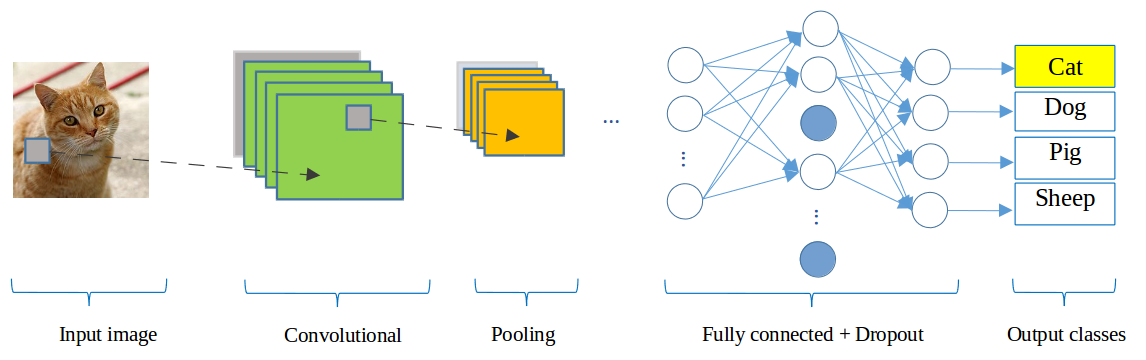
\includegraphics[scale=.3]{images/cnn_network_2}
	\caption{A CNN network for classification problem}
	\label{imgcnn_network}
\end{figure}

Convolutional (CONV) layer is used as a feature extractor by applying some learnable weights (filters) on the input images. The input image is convolved with the filters in order to compute the new feature maps; then, the convolved results are sent through a nonlinear activation before sending to the next layer. In CONV layer, the neurons are arranged into feature maps. All the neurons within a feature map have the same constraints; however, different features maps within the same CONV layer have different weights so that several features can be extracted at each location of an input image.

Pooling (POOL) layer is mostly used to down-sampling the size of the input with the purpose to reduce the spatial resolution of the feature map and so to reduce the computation cost. Initially, it was a common practice to use average pooling to propagate the average of all the inputs to the next layer. However, in more recent models \cite{krizhevsky2012imagenet, ciregan2012multi, li2015convolutional}, maximum pooling function has been prefered. It propagates the maximum values of the inputs to the next one. Fig. \ref{imgcnn_pooling} illustrates the differences between maximum and average pooling: Giving an input image of size $(4 \times 4)$, if applying a filter with size of $(2 \times 2)$ and a stride of $2$, if we apply to the yellow region an average pooling, the output will be $36.25$ and a maximum pooling will return the value $122$.
%However, the value in each element of the output is different because the max pooling outputs the maximum values of the filter region, while average pooling outputs the average value of the same region.

\begin{figure}[!h]
	\centering
	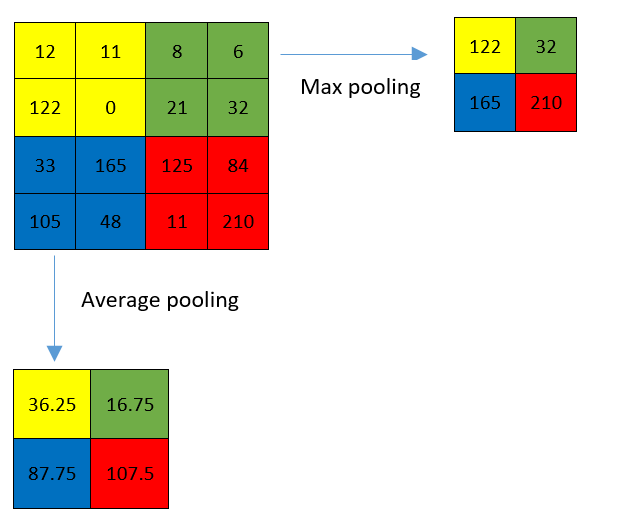
\includegraphics[scale=.5]{images/pooling}
	\caption{The results of different pooling}
	\label{imgcnn_pooling}
\end{figure}

Dropout (DROP) \cite{srivastava2014dropout} is a technique used to prevent the over-fitting during the training. The term dropout mentions dropping some output units and their connections (incoming and outgoing) belonging to a layer in the network. The units are dropped randomly with a probability $p$. When applying dropout technique, the network becomes a collection of thinned networks \cite{srivastava2014dropout}. So, training a neural network with dropout looks like training a collection of thinned networks. The dropouts layers are most often placed after the fully connected layers, but it is possible to use them after the pooling layers to introduce some kind of images noise augmentation.

Fully connected (FC) layer usually follows the group of convolutional and pooling layers to extract the abstract feature representations of the image. A CNN may have one or several FC layers. They interpret the feature representations (their inputs) and perform a function of high-level reasoning by applying the activation functions. In practice, the last fully connected layer produces the output of the network and choosing the activation function is depended on which kind of problem that network solves.

%From AlexNet period to ResNet-50, the obtained success stories \cite{krizhevsky2012imagenet,he2016deep} have proved that CNN models produce better results on a large dataset. To use this technique, the size of dataset remains as a bottleneck. Before to describe our proposed network architecture, we describe in the next section a way to augment data dedicated to our work.

\subsection{State of the arts in deep learning and key points detection}
LeNet \cite{lecun1998gradient} model is considered as the first architecture of CNN. LeCun et al. \cite{lecun1998gradient} have used LeNet to classify the handwritten digits in cheques. LeNet exhibits a standard architecture of a CNN which consists of convolutional layers, pooling layers, followed by two fully connected layers. But to be applied to realistic problems, this model requires huge computation capacities and a large amount of training data which are not available at the early 2000s. In the last ten years, as the capabilities to compute have been drastically improved and in the same time, a huge amount of data became available, new models of neural networks appear well adapted to this new environment. One of the first ones is AlexNet \cite{krizhevsky2012imagenet}, which is similar to LeNet \cite{lecun1998gradient} but with a deeper structure: LeNet has 2 convolutional layers and 1 fully connected layer while AlexNet has 5 and 3, respectively. Furthermore, in AlexNet the activation functions have been changed and dropout layers have been added to prevent the over-fitting. AlexNet won the famous ImageNet Challenge\footnote{This is a challenge where evaluates algorithms for object detection and image classification.} in 2012. From the success of AlexNet, a lot of different models have been proposed to improve the performance of CNN, one can cite ZFNet  \cite{zeiler2014visualizing}, GoogLeNet \cite{szegedy2015going}, VGGNet \cite{simonyan2014very}, or ResNet-50 \cite{he2016deep}. The main difference between these networks is that their architectures became deeper and deeper by adding more layers, e.g. ResNet-50, which won the champion of ILSVRC 2015, is deeper than AlexNet around $20$ times.
 
Besides classification or recognition of objects, CNNs have been also used to detect key points inside images. Liu et al. \cite{liu2016fashion} have presented a method to predict the positions of functional key points on fashion items such as the corners of neckline, hemline and cuff. Yi Sun et al. \cite{sun2013deep} have proposed a CNNs cascade to predict the facial points on the human face. 
Their model contains several CNNs which are linked together in a list as a cascade. Three levels of the cascade are set to recognize the human face from the global to local view with the objective to increase the accuracy of predicted key points. In the same topic, Zhanpeng Zhang et al. \cite{zhang2014facial} have proposed a \textit{Tasks-Constrained Deep Convolutional Network} to join facial landmarks detection problem with a set of related tasks, e.g. head pose estimation, gender classification, age prediction, or facial attribute inference. In their method, the input features have been extracted by $4$ convolutional layers, $3$ pooling layers and $1$ fully connected layer which is shared by  multiple tasks in the estimation step. Shaoli Huang et al. \cite{huang2017coarse} have introduced a coarse-fine network to locate keypoints and to estimate human poses. Their framework consists of the base convolutional layers shared by two streams of keypoint detectors: The first stream, named coarse stream, includes $3$ detector branches (3 stacks of Inception modules \cite{szegedy2015going}) which are used to focus on capturing local characteristics and modeling spatial dependencies between human parts. The second one, named fine stream, receives features which are concatenated from the coarse stream and provides the accurate localization. Cintas et al. \cite{cintas2016automatic} have introduced an architecture which is enable to recognize $45$ landmarks on human ears. Their proposed model includes a structure with $2$ convolutional layers, $1$ pooling layers, and $1$ dropout layer to extract the features. This structure is repeated $3$ times and is followed by 3 fully connected layers. In the same context of key point detection, we have developed a CNN to automatize landmarks prediction on beetle's anatomies. 

From AlexNet period to ResNet-50, the obtained success stories \cite{krizhevsky2012imagenet,he2016deep} have proved that CNN models produce better results on a large dataset. To use this technique, the size of dataset remains as a bottleneck. The next section is turn to the description of the method we have designed to augment the size of the dataset.
%As our work consists of a new architecture proposition for CNN, we have chosen to give in the next section some details about the definition of the different types of layers in CNN. The reader familiar to CNN can jump directly to the section about data augmentation.

\section{Data augmentation}
\label{Sdataaug}

The fundamentals of deep learning algorithms are to train the models on dataset repeatedly in order to reach the best accuracy. So, providing a large dataset asserts to learn more cases and clearly improves the learnable of the network. Unfortunately, in some application domains as in biology, providing large dataset is costly and could be difficult to obtain. For this reason, one way to solve this problem is to create misshapen data from real data and to add them to the training set. Most often in image processing, dataset augmentation uses operations like translation, rotation or scaling which are well known to be efficient to generate new version of existing images. However, this kind of operations are not useful in our case because the analysis of images by CNN (convoluted) are most often invariant to translation or rotation. So, we have designed another method to obtain misshapen images.

Our image set is in RGB color map, the first procedure consists of changing the value of one color channel of the three channels in the original image to generate a new image. A constant value is sampled in an uniform distribution $\in [1, N]$ to obtain a new value caped at $255$. For example, Fig. \ref{figaug1} shows the three images which are generated  when a constant $c = 10$ is added to each channel of an original image. Following this way, we can generate three new versions of only one image.

\begin{figure}[h]
	\centering
	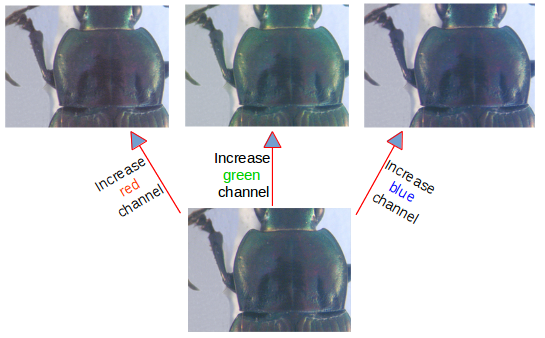
\includegraphics[scale=0.4]{images/inc_channels}
	\caption{A constant $c = 10$ has been added to each channel of an original image}
	\label{figaug1}
\end{figure}

In the second procedure, each channel is considered separately and one gray image is generated for it (Fig. \ref{figaug2}). Consequently, we obtain 3 new images (single channel) from an original one. At the end of the process, $6$ versions of an original image are made. In total, the new data set contains $293 \times 7 = 2051$ images for each anatomical part of beetle (an original image and six misshapen ones).

\begin{figure}[h]
	\centering
	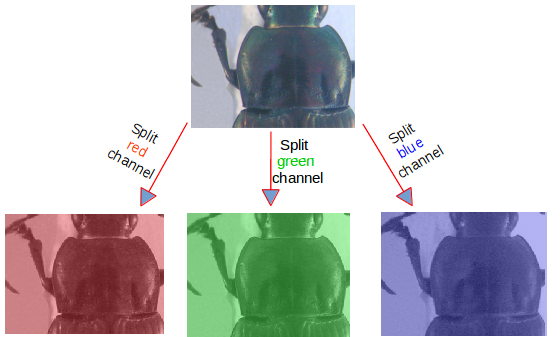
\includegraphics[scale=0.4]{images/sp_channels}
	\caption{Three channels (red, green, blue) are separated from original image}
	\label{figaug2}
\end{figure}
%However, we have not used all images for training and validation. So, we have chosen $260$ original images and their generations ($1820$ images) of each dataset for training and validation processes, the remaining images ($33$ original images) are used for test process. In practical, to obtain a fast convergence during the computing, it is useful to normalize the brightness of the images to $[0,1]$ instead of $[0, 255]$ and the coordinates of the landmarks have been also normalized \cite{lecun2012efficient}.

\section{Network architectures designing}
\label{Sneuralnetwork}
As we have presented previously, several CNN architectures are available from literature and tools libraries. It is always possible to adapt them to a specific application by changing the parameters values or by modifying the arrangement of layers. By the way, several trials have been achieved before to obtain a satisfying model dedicated to landmarks estimation. In this section, we present three versions of the model that we have designed to solve this task. As usual, we have combined the classical layer types to build the model, i.e., convolutional, maximum pooling, dropout, and full-connected layers.

The first architecture has been a very classical one (Fig. \ref{fignet1}). It receives an input image with the size of $(1 \times 192 \times 256)$, then it is composed by three repeated structures of a convolutional (CONV) layer followed by a maximum pooling (POOL) one. In most of CNNs, the parameters of CONV layers have been set to increase the depth of the images from the first  to the last layer. This is done by setting the number of filters at each CONV layer. In this first model, the depths of the CONV layers increase from $32, 64, $ to $128$ and with different size of the kernels: $(3 \times 3)$, $(2 \times 2)$ and $(2 \times 2)$, respectively. Inserting POOL layers after a convolutional layers is usually done. The POOL layer effects to progressively reduce the spatial size of the representation to reduce the number of parameters, computation in the network, and also to control over-fitting. The operation of POOL layers is independent for each depth slice of their inputs. In our model, we have used the most common form for one POOL layer: a filter with size of $(2 \times 2)$ and a stride of $2$ pixels. At the end of the model, three FC layers have been added to extract the global relationship between the features and to proceed the outputs. The first two FC layers have been applied the activation functions to make sure these nodes interact well and to take into account all possible dependencies at the feature level. The outputs of the FC layers are $500, 500$ and $16$. The output of the last FC layer corresponds to the coordinates ($x$ and $y$) of $8$ landmarks which we would like to predict. Nevertheless, the obtained results with this architecture has not been considered as enough good to continue to use it. One of the main problems is the presence of over-fitting during the training process (Detailed results will be discussed in Section \ref{sexperiments}).

\begin{figure}[!h]
	\centering
	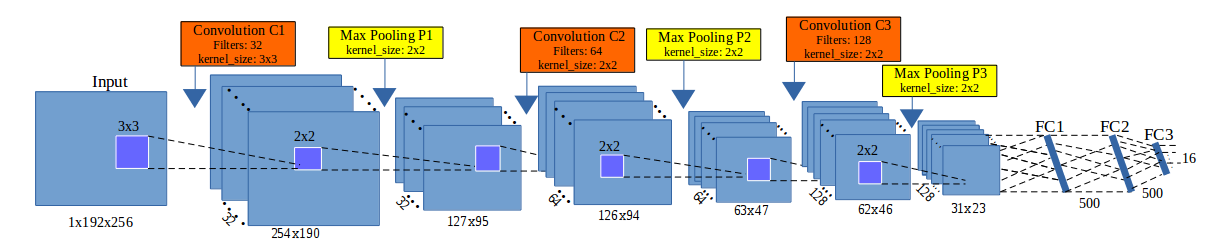
\includegraphics[scale=0.3]{images/net1}
	\caption{The architecture of the first model}
	\label{fignet1}
\end{figure}

The second model has kept the same architecture but the number of output of the two FC layers has been increased to $1000$. Increasing the value at FC layers could allow to get more features from CONV layer without requirements of computing resources. However, the obtained results remained not satisfying, it will be discussed in the result section (Section \ref{sexperiments}). 

To build the third architecture, we have defined a new concept: the \textit{elementary block}. An {elementary block} is defined as a sequence of a CONV ($C_{i}$), a maximum POOL ($P_i$) and a dropout ($D_i$) layers (Fig. \ref{figelementary}). The Dropout layer has been added to prevent over-fitting by addition of a step of removal of some nodes. This significantly reduces overfitting and gives major improvements over other regularization methods \cite{srivastava2014dropout}. The final architecture is a composition of elementary blocks. 
%The idea of dropout is to include some variations between different runs. During training phase, dropout samples are done from an exponential number of different ``thinned" network. At test phase, it is easy to approximate the effect of averaging the prediction of all thinned networks by simply using a single unthinned network with smaller weights.
\begin{figure}[h]
	\centering
	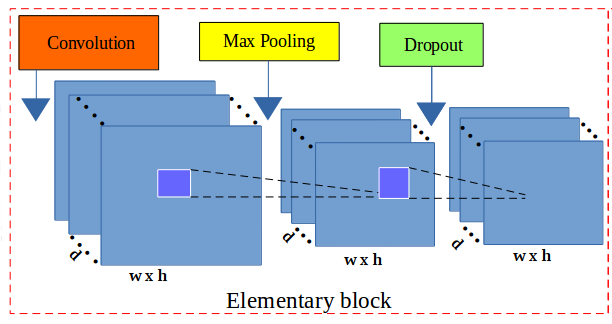
\includegraphics[scale=0.3]{images/elementary_block}
	\caption{The layers in an elementary block. It includes a CONV layer (red), a maximum POOL layer (yellow) and a DROP layer (green).}
	\label{figelementary}
\end{figure}

Fig. \ref{fignet3} illustrates the layers in the third architecture. For our purpose, we have assembled \textbf{3 elementary blocks}, the main components of \textbf{EB-Net}. The parameters for each layer in each elementary block are described as below, the list of values follows the order of elementary blocks ($i = [1..3]$):
\begin{itemize}
	\item CONV layers:
	\begin{itemize}
		\item Number of filters: $32, 64, $ and $128$
		\item Kernel filter sizes: $(3 \times 3), (2 \times 2), $ and $(2 \times 2)$
		\item Stride values: $1, 1, $ and $1$
		\item No padding is used for CONV layers 
	\end{itemize}
	\item POOL layers:
		\begin{itemize}
			\item Kernel filter sizes: $(2 \times 2), (2 \times 2), $ and $(2 \times 2)$
			\item Stride values: $2, 2, $ and $2$
			\item No padding is used for POOL layers
		\end{itemize}
	\item DROP layers:
		\begin{itemize}
			\item Probabilites: $0.1, 0.2, $ and $0.3$
		\end{itemize}
\end{itemize}

Three FC layers are kept the same as the second architecture: FC1 and FC2 have $1000$ outputs, the last FC layer (FC3) has $16$ outputs. As usual, a dropout layer is inserted between FC1 and FC2 with a probability equal to $0.5$.
\begin{figure}[h]
	\centering
	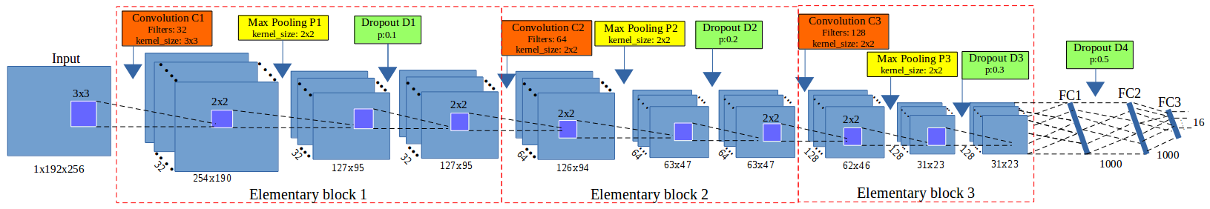
\includegraphics[scale=0.3]{images/net3}
	\caption{The architecture of EB-Net}
	\label{fignet3}
\end{figure}

The core of CNN is training over iteration. There are many ways to optimize the learning algorithm, but gradient descent \cite{lecun2012efficient} is currently a good choice to reduce the loss in neural network. The core idea is to follow the gradient until to reach stable state. So, we have chosen gradient descent in the backward phase to update the values of learnable parameters and to increase the accuracy of the network. The networks are designed to use the same learning rate and a momentum. The learning rate is initialized at $0.03$ and stopped at $0.00001$, while the momentum is updated from $0.9$ to $0.9999$. Their values are updated over training time to fit with the number of epochs \footnote{An epoch is a single pass through the full training set} by applying parameters adjustment during the training. The three architectures implementations have been done on Lasagne framework \cite{lasagne} by Python code. More information about the model can be obtained from the repository on GitHub: \texttt{https://github.com/linhlevandlu/CNN\_Beetles\_Landmarks}

\section{Experiments and results}
\label{sexperiments}
This work is a part of a project about automatized morphology. The choice to turn to deep learning process has been motivated by the high difficulty to segment some parts of the beetle images and consequently to apply classical image processing methods. The pronotum was the first part we have analyzed with deep learning. The networks have been trained in $5, 000$ epochs on Linux OS by using NVIDIA TITAN X cards. During the training, the images are chosen randomly from the dataset with a ratio of $60\%$ for training and $40\%$ for validation. For each image, a set of $8$ manual landmarks are available. They have been set by biologists and are considered as the ground truth for the evaluation. In deep learning, many kinds of loss expressions can be considered depending on the class of problem solving by the network, for example, Root Mean Square Error (RMSE) is usually used for regression problems where the outputs are not discrete values. In the context of deep learning, landmark prediction can be seen as a regression problem because the coordinates of landmarks do not belong to discrete classes. Therefore, RMSE has been used to compute the losses of architectures during the training process. 
%At the test phase, images without landmarks are given to the trained network to produce output coordinates of the predicted landmarks. The results then evaluated by comparing with the manual landmarks coordinates provided by biologists which have been seen as ground truth. 

\begin{figure}[htbp]
    \centering
    \subfloat[The first model]{\label{figloss1}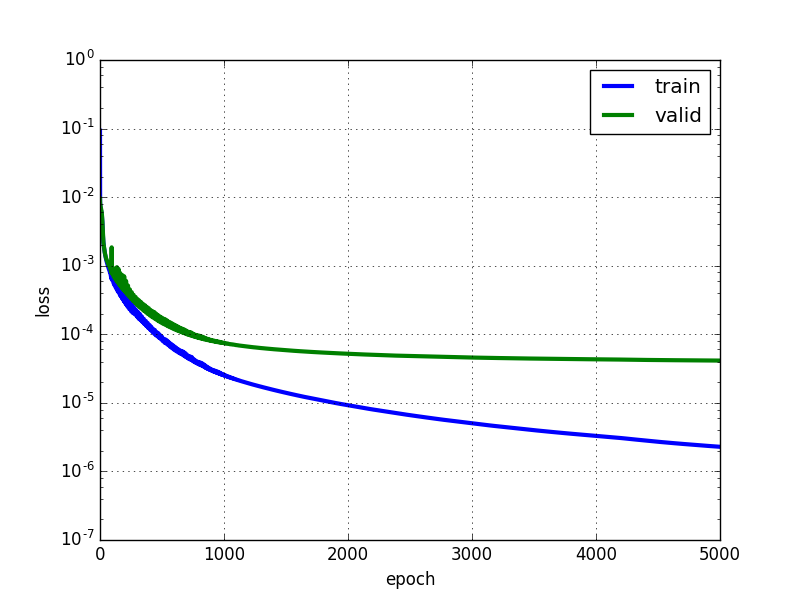
\includegraphics[scale=0.3]{images/model1_loss}}~~
\subfloat[The second model]{\label{figloss2}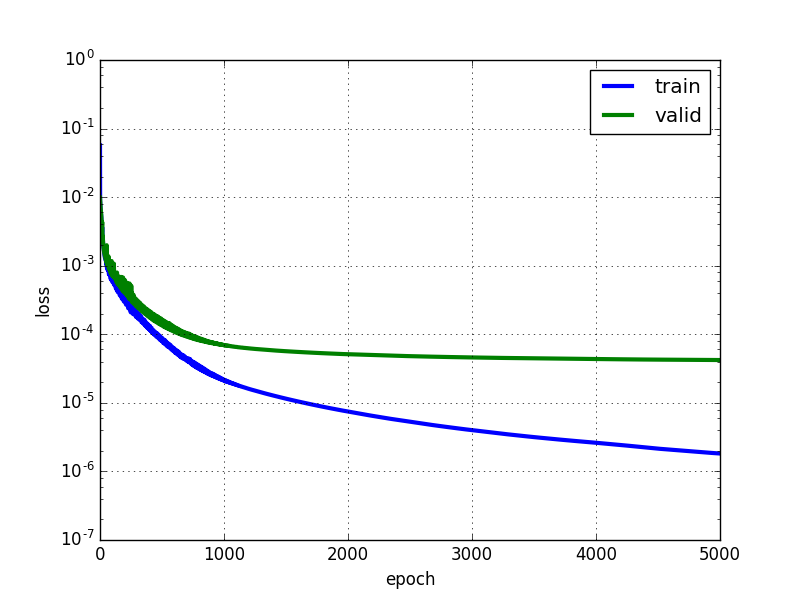
\includegraphics[scale=0.3]{images/model2_loss}}\\    
    \caption{The losses (training and validation) of the models}
    \label{figlosses}
\end{figure}

Fig. \ref{figloss1} shows the training errors and the validation errors during training phase of the first architecture. The blue curve presents the RMSE errors of training process while green curve is the validation errors. Clearly, over-fitting has appeared in the first model, i.e., training losses are able to decrease but validation losses are stable. In the second model (Section \ref{Sneuralnetwork}), the parameters of full-connected layers have been modified to prevent the over-fitting but it seems that this solution is still not satisfying, the results are very similar to the previous ones (over-fitting is still appears).

Fig. \ref{figloss3} illustrates the losses during the training of the third model, one can note that after several epochs, the two-loss values become closed and the over-fitting disappears.  The sequence of Dropout addition inside elementary block works well to prevent over-fitting and improve the accuracy of the model greatly. This third model has been selected to compute automatically landmarks.

\begin{figure}[htbp]
    \centering
    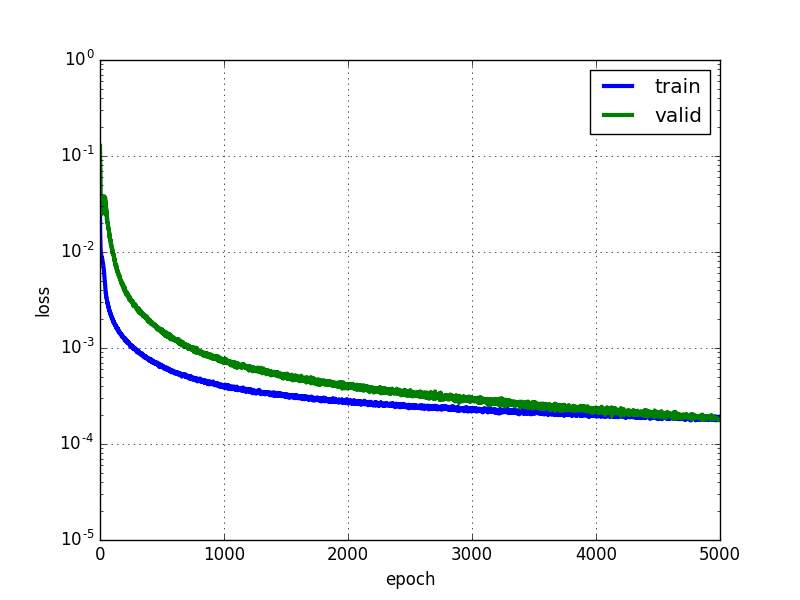
\includegraphics[scale=0.35]{images/model3_loss}
    \caption{The losses (training and validation) of the third model}
    \label{figloss3}
\end{figure}

In order to extract predicted landmarks from all pronotum images, we have applied \textit{cross-validation} procedure to choose the test images, we call it \textit{round}. For each round, we have decided to choose $33$ images for testing step. In order to predict landmarks for all available images, we will do $9$ rounds. The $260$ remaining images are used as training and validation images. Of course, this dataset will be augmented as described before to provide $1820$ images for these $2$ steps. Table. \ref{tbltrainingloss} resumes the losses of $9$ rounds when we trained the third model on pronotum images. Clearly, the training/validation loss among rounds are tiny and stable.

\begin{table}[h!]
	\centering
	\begin{tabular}{l l l}
	Round & Training loss & Validation loss \\ \hline
	1 & 0.00018 & 0.00019  \\ \hline
	2 & 0.00019 & 0.00021 \\ \hline
	3 & 0.00019 & 0.00026 \\ \hline
	4 & 0.00021 & 0.00029 \\ \hline
	5 & 0.00021 & 0.00029 \\ \hline
	6 & 0.00019 & 0.00018 \\ \hline
	7 & 0.00018 & 0.00018 \\ \hline
	8 & 0.00018 & 0.00021 \\ \hline
	9 & 0.00020 & 0.00027 \\ \hline
	\end{tabular}
	\caption{\small{The losses during training the third model on pronotum images}}
	\label{tbltrainingloss}
\end{table}

To evaluate the coordinates of predicted landmarks, the correlation metrics between the manual landmarks and corresponding predicted ones have been computed. Table. \ref{tblcorrelation} shows the correlation scores of $3$ metrics (using \textit{scikit-learn} \cite{pedregosa2011scikit}), e.g. coefficient of determination ($r^2$), explained variance (EV), and Pearson correlation. These three metrics are both appropriate for our dataset type. The results closed to $1$ show that the predicted coordinates are very close with the ground truth. It proves that our prediction is good enough to replace manual landmarks in statistical analysis of pronotum morphology. However, standing on the side of image processing, seeing the real coordinates on images is more appropriate than statistical results. So, the distances (in pixels) between manual coordinates and predicted coordinates have been calculated for all images. Then, the average distance for each landmark has been computed.

\begin{table}[htbp]
	\centering
	\begin{tabular}{|c|p{2cm}|p{2cm}|p{2cm}|}
		\hline
		Metric & $\mathbf{r^{2}}$ & \textbf{EV} & \textbf{Pearson} \\ \hline
		Score & $\textbf{0.9952}$ & $\textbf{0.9951}$ & $\textbf{0.9974}$ \\\hline
	\end{tabular}
	\caption{Correlation scores between manual landmarks and predicted landmarks}
	\label{tblcorrelation}
\end{table}

Table. \ref{tblavgpronotum} shows the average distances by landmarks on all images of pronotum dataset. With the images resolution $256 \times 192$, we can consider that an error of $1\%$ (corresponding to $2$ pixels) could
be an acceptable error. Unhappily, our results exhibit average
distance of $4$ pixels in the best case, landmark $1$ and more than
$5$ pixels in the worse case, landmark $6$.

\begin{table}[htbp]
	\centering	
	\begin{tabular}{|c|c|}
		\hline
		\textbf{Landmark} & \textbf{Distance} (in pixels) \\ \hline
		1 & \textcolor{green}{\textbf{4.002}}  \\ \hline
		2 & 4.4831 \\ \hline
		3 & 4.2959 \\ \hline
		4 & 4.3865 \\ \hline
		5 & 4.2925 \\ \hline
		6 & \textcolor{red}{\textbf{5.3631}} \\ \hline
		7 & 4.636 \\ \hline
		8 & 4.9363 \\ \hline
	\end{tabular}
	\caption{The average distances on all images per landmark on pronotum images.}
	\label{tblavgpronotum}
\end{table}

Fig. \ref{figchartlm1} shows the distribution of the distances on the first landmark of all images. The accuracy based on the distance in each image can be
separated into three spaces: best results, the images having distance less
than the average value ($4$ pixels): $56.66\%$; acceptable results, the images having the
distance from the average value to $7$ pixels (standard deviation error): $31.40\%$; and the images which are clearly in error with the distance greater than $7$ pixels: $11.94\%$.

\begin{figure}[htbp]
	\centerline{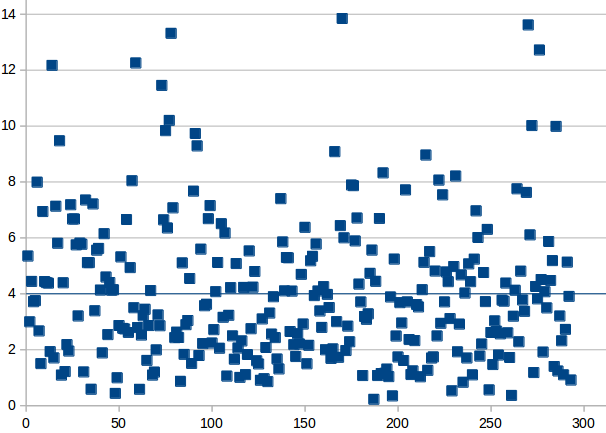
\includegraphics[scale=0.3]{images/statistic_pronotum_from_scratch_lm1}}
	\caption{The distribution of the distances on the first landmark. The blue line is the average value of all distances.}
	\label{figchartlm1}
\end{figure}

To illustrate this purpose, Fig. \ref{figrsexample} shows the predicted landmarks on two test images. One can note that even some predicted landmarks (Fig. \ref{figsub1}) are closed to the manual ones, in some case (Fig. \ref{figsub2}) the predicted ones are far from the expected results. So, the next step has been dedicated to the improvement of these results.
%This result explains why the average distance by landmarks are enough good while some predicted landmarks are so far from the manual one.
\begin{figure}[htbp]
    \centering
    \subfloat[Image with well-predicted landmarks]{\label{figsub1}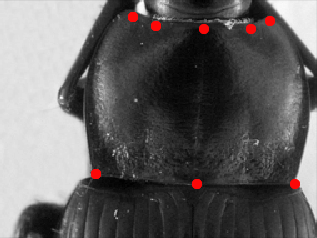
\includegraphics[width=0.35\textwidth]{images/fn_accuracy}}~~
\subfloat[Image with inaccuracy landmarks]{\label{figsub2}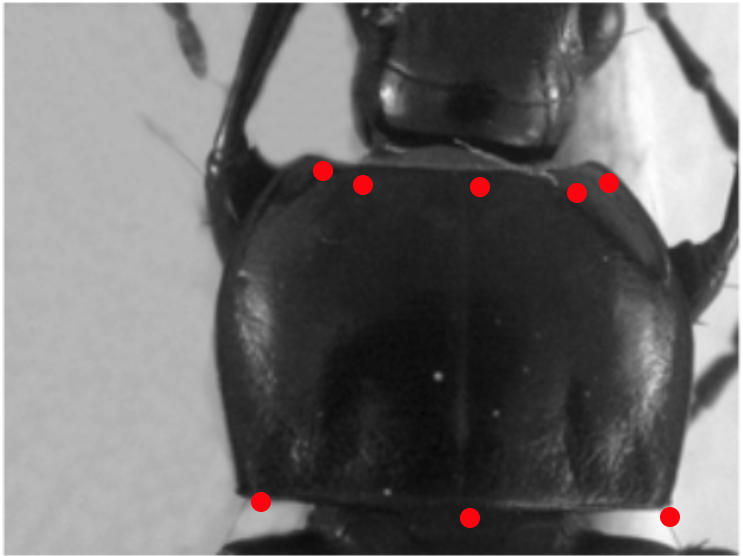
\includegraphics[width=0.35\textwidth]{images/plandmark2}}\\    
    \caption{The predicted landmarks, in red,  on the images in test set.}
    \label{figrsexample}
\end{figure}
\section{Resulting improvement by fine-tuning}
\label{sfineTuning}
EB-Net, which was presented in Section \ref{Sneuralnetwork}, have been trained from scratch on five datasets of beetles (left mandible, right mandible, pronotum, elytra, and head). At that step, the network was able to predict the landmarks on the images. But as we have discussed, even if the strength of the correlation seems to validate the results, when we display the predicted landmarks on the images, the quality of the predicted coordinates are not enough precise, and the average distances are a little bit high.

Training a network from scratch is not the only way to work in Deep learning. It is possible to initialize parameter values with values extract from another experiment on another dataset. It is called transfer learning \cite{torrey2009transfer}. Transfer learning aims
to address the problem when the distribution of the training
data from the source domain is different from that of the future data from the target domain \cite{lin2016homemade}. In order to improve our results, we have broadened model with this technique. In the idea, the obtained parameters values of a model, which have been used to solve a problem, are reused on other datasets \cite{margeta_mri}. The name of this procedure is currently called \textbf{fine-tuning}.

Fine-tuning does not only replace and retrain the last layer of the model on
the new dataset but also fine-tunes the weights of a trained
model by continuing the backpropagation. In deep learning domain, ImageNet \cite{imagenet_cvpr09} is a well-known dataset with more than $100,000 $ images. It has been used to train many famous CNN architectures such as AlexNet \cite{krizhevsky2012imagenet}, VGG-16 \cite{simonyan2014very}, which have achieved the large success. The pre-trained models on ImageNet then have been shared in deep learning community as a source for the researcher who would like to continue using the features of ImageNet. Unfortunately, some preliminary tests have shown that re-using ImageNet features
is not relevant for our application because landmarks detection has a difference from image recognition. On the other hand, we noticed that our problem is related to face recognition and facial keypoints detection. So, we have decided to train our model on a facial keypoints dataset which is considered as a source domain. Then, the trained parameters are transfered to predict landmarks on beetle's images as target domain.

%We have designed a way to reproduce the method with our own data. It is worth noting that of course the size of the dataset to pre-train was not at all no huge than this one of ImageNet. To finish this task, we have pre-trained our model on another task (facial keypoints detection) before applying to fine-tune on each part of beetle. 

\subsection{Pre-train model architecture with facial keypoints dataset}
\textbf{Facial keypoints dataset} has been published on Kaggle community \footnote{https://www.kaggle.com/c/facial-keypoints-detection} by University of Montreal. It includes $2,140$ human face images with the size of $96 \times 96$. Each image contains $15$ landmarks on the face: $6$ landmarks for eyes, $4$ landmarks for eyebrows, $4$ landmarks for mouth, and $1$ landmarks for nose tip. Fig. \ref{figaface} shows four face images in the dataset and the landmarks on each the face.

\begin{figure}[htbp]
	\centerline{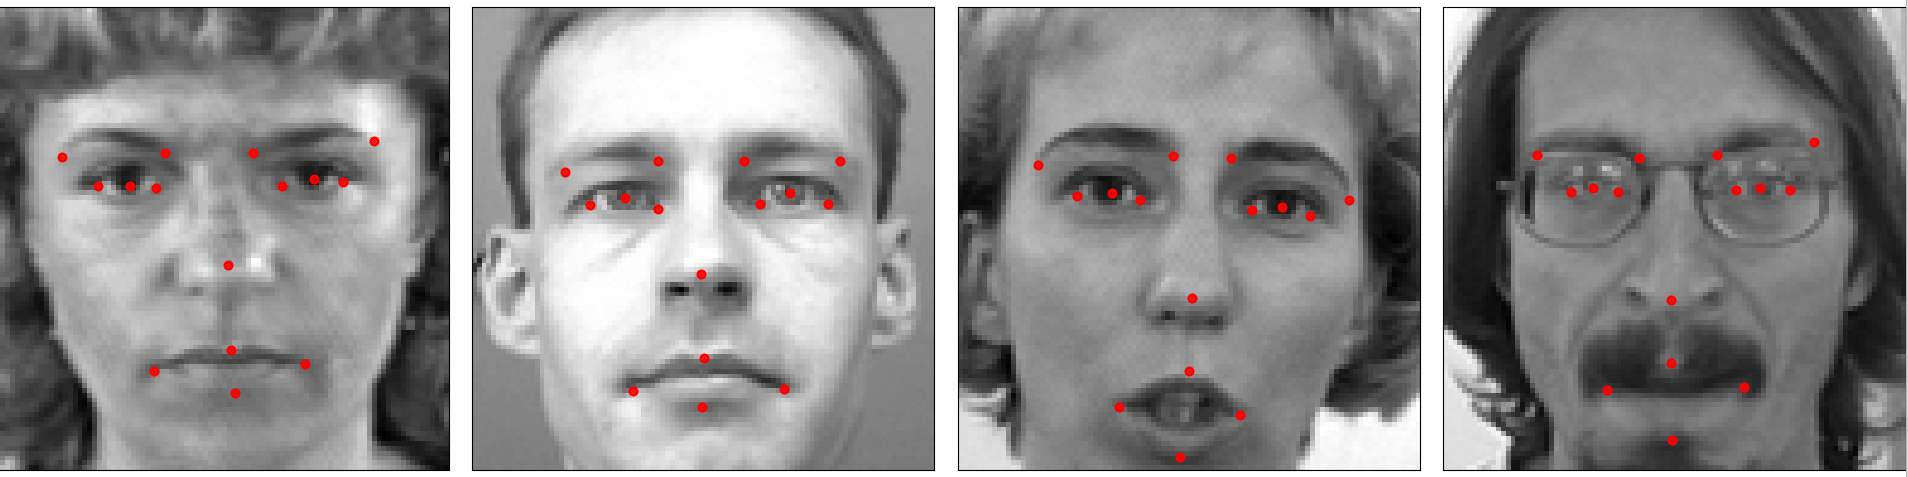
\includegraphics[scale=0.16]{images/face_dataset_2.png}}
	\caption{Four face images in the dataset and ground truth position of the landmarks.}
	\label{figaface}
\end{figure}

For the pre-training step, EB-Net continues to be selected to train the facial keypoint dataset instead of using other models. The objective of this task is to evaluate and to compare the effectiveness of EB-Net and other promotions in the challenge. Basically, the architecture parameters (number filters, size of filter, padding, stride) are the same as working on beetle's parts. We have just changed the input size of network model to $96 \times 96$ and the output of the last FC layers to correspond to the number of landmarks ($15$ landmark). For hyper-parameters of model, the learning rate and momentum have been remained the same. However, the number of epochs have been changed to $10,000$ instead of $5,000$ to achieve better learning on the parameters. After training, the RMSE\footnote{RMSE: Root Mean Square Error} score that obtained is $1.1464$. This score is better than top $3$ on the leader board of challenge. It proved that EB-Net fits perfectly with facial keypoints challenge and we have good reason to believe that the obtained parameter values of EB-Net on facial keypoints dataset can use to fine-tune on beetle's images.
\subsection{Fine-tuning on each beetle's part}
EB-Net has been pre-trained on facial keypoints dataset with $30$ outputs ($15$ landmarks). Then, the parameters have been transfered to fine-tune on the images of each beetle's part. The fine-tuning stage has been done by continuing the backpropagation to update the layers parameters.

In another scene, to be able to use the same parameters for fine-tuning process, the input images have been cropped to suppress the part which are empty, to obtain a new image size of $192 \times 192$; and a modification was made on stride properties of the first convolutional layer (changing from $1$ to $2$).

During fine-tuning, cross-validation has been applied to select data for training and validation. After finishing the fine-tuning process, EB-Net was used to predict the landmarks on test images. To evaluated the accuracy of the model's output, the distances (in pixels) between predicted and corresponding manual landmarks have been calculated. Then, the average distances have been computed based on the distances. Tables. \ref{cmppronotum}, \ref{cmptete}, \ref{cmpelytre}, \ref{cmpmg}, and \ref{cmpmd} show the average distances by landmarks on each beetle's part of two processes: training from scratch and fine-tuning process. \textbf{From scratch} columns remind the previously average distances when EB-Net was trained from scratch. \textbf{Fine-tune} columns present the new average distances after applying fine-tuning on each part. The green and red values represent the best and the worst average distances on each part. From these tables, there is a difference in average distances between two process, the average distances of each landmark has decreased in the case of fine-tuning. It is clearly proved that the quality of predicted landmarks with the help of fine-tuning is more precise than training from scratch.
\begin{table}[htbp]
	\centering
	\begin{tabular}{|c|c|c|}
		\hline
		\textbf{$\#$LM} & \textbf{From scratch} & \textbf{Fine-tune} \\ \hline
		1 & \textcolor{green}{\textbf{4.00 }}& 2.99\\ \hline
		2 & 4.48 & 3.41  \\ \hline
		3 & 4.30  & 2.98 \\ \hline
		4 & 4.39  & 3.54\\ \hline
		5 & 4.29  & 3.37 \\ \hline
		6 & \textcolor{red}{\textbf{5.36}}  & \textcolor{red}{\textbf{4.06}} \\ \hline
		7 & 4.64  & \textcolor{green}{\textbf{2.93}} \\ \hline
		8 & 4.94  & 3.64 \\ \hline
	\end{tabular}
	\caption{Average distances comparison between training from scratch and fine-tuning on pronotum images}
	\label{cmppronotum}
\end{table}

\begin{table}
	\begin{minipage}[t]{0.45\textwidth}
		\centering
		\begin{tabular}{|c|c|c|}
		\hline
		\textbf{$\#$LM} & \textbf{From scratch} & \textbf{Fine-tune} \\ \hline
		1 & \textcolor{red}{\textbf{5.53}} & \textcolor{red}{\textbf{4.82}}\\ \hline
		2 & 5.16 & 4.21 \\ \hline
		3 & 5.38  & 4.73 \\ \hline
		4 & 5.03  & 4.11 \\ \hline
		5 & \textcolor{green}{\textbf{4.18}}  & \textcolor{green}{\textbf{2.76}}\\ \hline
		6 & 4.45  & 3.50 \\ \hline
		7 & 4.79  & 3.92 \\ \hline
		8 & 4.53  & 3.40\\ \hline
		9 & 5.14  & 4.17 \\ \hline
		10 & 5.06  & 3.94\\ \hline
	\end{tabular}
	\caption{Average distances comparison between training from scratch and fine-tuning on head images}
	\label{cmptete}
	\end{minipage}
	\hfill
	\begin{minipage}[t]{0.45\textwidth}
		\centering
		\begin{tabular}{|c|c|c|}
			\hline
			\textbf{$\#$LM} & \textbf{From scratch} & \textbf{Fine-tune} \\ \hline
			1 & \textcolor{green}{\textbf{3.87}} & 3.21  \\ \hline
			2 & 3.97 & 3.28 \\ \hline
			3 & 3.92  & \textcolor{green}{\textbf{3.20}}\\ \hline
			4 & \textcolor{green}{\textbf{3.87}}  & 3.22 \\ \hline
			5 & 4.02  & 3.31 \\ \hline
			6 & 4.84  & 4.21\\ \hline
			7 & 5.21  & 4.54 \\ \hline
			8 & \textcolor{red}{\textbf{5.47}}  & \textcolor{red}{\textbf{4.76}}\\ \hline
			9 & 5.27  & 4.55 \\ \hline
			10 & 4.07  & 3.39 \\ \hline
			11 & 3.99  & 3.29 \\ \hline
		\end{tabular}
		\caption{Average distances comparison between training from scratch and fine-tuning on elytra images}
		\label{cmpelytre}
	\end{minipage}
\end{table}
\begin{table}
	\begin{minipage}[t]{0.45\textwidth}
		\centering
		\begin{tabular}{|c|c|c|}
			\hline
			\textbf{$\#$LM} & \textbf{From scratch} & \textbf{Fine-tune} \\ \hline
			1 & \textcolor{red}{\textbf{9.13}} & 5.28 \\ \hline
			2 & \textcolor{green}{\textbf{6.72}} & 4.05 \\ \hline
			3 & 6.87 & 4.01 \\ \hline
			4 & 6.77 & 4.02 \\ \hline
			5 & 7.13 & 3.92 \\ \hline
			6 & 6.94 & \textcolor{green}{\textbf{3.88}} \\ \hline
			7 & 7.32 & 4.01 \\ \hline
			8 & 7.41 & 4.16 \\ \hline
			9 & 7.58 & 4.35 \\ \hline
			10 & 7.63 & 4.46 \\ \hline
			11 & 7.69 & 4.72 \\ \hline
			12 & 8.42 & 5.08 \\ \hline
			13 & 7.99 & 4.50 \\ \hline
			14 & 7.49 & 4.26 \\ \hline
			15 & 7.79 & 4.62 \\ \hline
			16 & 8.52 & \textcolor{red}{\textbf{6.04}} \\ \hline
		\end{tabular}
		\caption{Average distances comparison between training from scratch and fine-tuning on left mandible images}
		\label{cmpmg}
	\end{minipage}
	\hfill
	\begin{minipage}[t]{0.45\textwidth}
		\centering
		\begin{tabular}{|c|c|c|}
\hline
\textbf{$\#$LM} & \textbf{From scratch} & \textbf{Fine-tune} \\ \hline
		1 & \textcolor{red}{\textbf{9.50}} & 4.86 \\ \hline
	2 & 7.17 & 4.06\\ \hline
	3 & 7.24 & 3.97\\ \hline
	4 & \textcolor{green}{\textbf{7.04}} & 3.87 \\ \hline
	5 & 7.16 & 4.05  \\ \hline
	6 & 7.57 & 3.82  \\ \hline
	7 & 7.43 & \textcolor{green}{\textbf{3.77}}  \\ \hline
	8 & 7.66 & 3.87  \\ \hline
	9 & 7.79 & 3.96 \\ \hline
	10 & 8.02 & 3.97 \\ \hline
	11 & 8.31 & 4.27 \\ \hline
	12 & 8.16 & 4.42 \\ \hline
	13 & 8.89 & 4.87 \\ \hline
	14 & 9.18 & 4.93 \\ \hline
	15 & 8.79 & 4.46 \\ \hline
	16 & 8.31 & 4.17 \\ \hline
	17 & 8.29 & 4.57 \\ \hline
	18 & 8.89 & \textcolor{red}{\textbf{5.89}} \\ \hline
		\end{tabular}
		\caption{Average distances comparison between training from scratch and fine-tuning on left mandible images}
		\label{cmpmd}
	\end{minipage}
\end{table}
In order to get a better view about predicted landmarks, we have calculated other statistical indicators such as median, standard error, minimum value and maximum value on each landmark based on the distances between predicted and corresponding manual landmarks. All statistical values and the distribution graphs are presented in \ref{appdixA}. From these tables, the minimum and the maximum distances have a large difference in all cases. However, the median values, which separate the set into two parts, are very close with minimum values and so far from maximum values, even smaller than the mean distances. It confirms that almost distances stay around the median values and the predicted landmarks are good enough to replace the manual ones. Besides, the distribution of the distances on each landmark of each part have been taked into account in \ref{appdixB}. We can observe that most of distances are close with the mean and median values, only some exceptional cases. Fig. \ref{figpdl} shows the predicted landmarks of fine-tuning process in one case of each part.

\begin{figure}[htbp]
    \centering
    \subfloat[Pronotum]{\label{}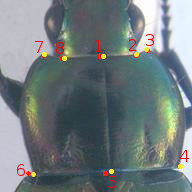
\includegraphics[width=0.45\textwidth]{images/predicted/Prono_001.JPG}}~~
    \subfloat[Head]{\label{}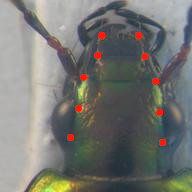
\includegraphics[width=0.45\textwidth]{images/predicted/Tete_005.JPG}}\\
    \subfloat[Left mandible]{\label{}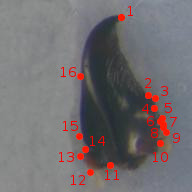
\includegraphics[width=0.45\textwidth]{images/predicted/Mg_001.JPG}}~~
    \subfloat[Right mandible]{\label{}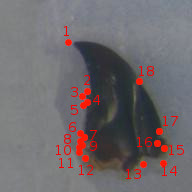
\includegraphics[width=0.45\textwidth]{images/predicted/Md_002.JPG}}\\
	\subfloat[Elytra]{\label{}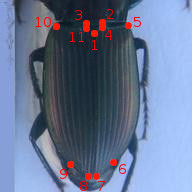
\includegraphics[width=0.45\textwidth]{images/predicted/Elytre004.JPG}}
    \caption{The location of predicted landmarks (red points) in one case of each part }
    \label{figpdl}
\end{figure}

The fine-tuning process has improved the results of the proposed architecture on both $5$ datasets: left, right mandible, pronotum, elytra and head. All the average distances have significantly decreased: $\approx 41.35\%$ on left mandible, $\approx 46.51\%$ on right mandible, $\approx 25.98\%$ on pronotum, $\approx 15.8\%$ on elytra, and $\approx 18.10\%$  on head part based on considering the average distances per landmark. Besides, if we consider a predicted point which has the distance (from manual ones) less than mean value plus standard deviation is acceptable, the accuracy of method on each part is $\textbf{87.07\%}$ on pronotum, $\textbf{87.92\%}$ on head, $\textbf{91.78\%}$ on elytra, $\textbf{93.58\%}$ on left mandible and $\textbf{88.31\%}$ on right mandible.

For segmentable images, we have a comparison between the results of deep learning and early method where we have applied image processing techniques to predict the landmarks \cite{le2017maelab}. Clearly, the result with fine-tuning has improved the location of estimated landmarks. Even the average distances which obtained from scratch training are still high but they are more stable than the results from the early method: most of the average distance(or landmarks) of left mandibles are less than the results of the early method, while the average distances are very closed in the case of right mandibles.
%\pagebreak
\section{Conclusion}
\label{sconclusion}
In this work, we have presented how to apply convolutional neural network to predict the landmark on 2D anatomical images of beetles. After going through many trial models, we have presented a convolutional neural network for automatic detection landmarks on anatomical images of beetles which includes the repeated of some elementary blocks (an elementary block consists of a convolutional layer, a max pooling layer, and a dropout layer) followed by fully connected layers. Then, the proposed model have been trained and tested by using two strategies: \textit{train from scratch} and \textit{fine-tuning}. 

In our case, the size of dataset is limited. Therefore, we have applied the image processing techniques to augment dataset. The predicted landmarks have been evaluated by calculating the distance between manual landmarks and corresponding predicted landmarks. Then, the average of distance errors on each landmarks has been considered.

The results have been shown that using the convolutional network to predict the landmarks on biological images leads to satisfying results without need for segmentation step on the object of interest. The
best set of estimated landmarks has been obtained after a step
of fine-tuning using the whole set of images that we have for the
project, i.e. about all beetle parts. The quality of prediction allows using automatic landmarking to replace the manual ones.
\section*{References}

\bibliography{includes/mybibfile}

\pagebreak
\appendix
\section{Statistic information on each beetle's part}
\label{appdixA}
Table \ref{a1}, \ref{a2}, \ref{a3}, \ref{a4}, and \ref{a5} show the statistical values on each part. The green and red numbers represent the best and the worst values on each statistical indicators, respectively.  
\begin{table}[htbp]
\begin{tabular}{ | c | c | c | c | c | c | }
\hline
	\textbf{\#LM} & \textbf{Mean} & \textbf{Standard Error} & \textbf{Median} & \textbf{Minimum} & \textbf{Maximum} \\ \hline
	LM1 & 2.9914 & \textcolor{green}{\textbf{0.1057}} & 2.7031 & \textcolor{red}{\textbf{0.23}} & 14.2496 \\ \hline
	LM2 & 3.4066 & 0.1306 & 2.9626 & 0.175 & 18.4053 \\ \hline
	LM3 & 2.9829 & 0.1205 & 2.5864 & 0.216 & 19.2092 \\ \hline
	LM4 & 3.5449 & 0.1422 & 3.117 & 0.1638 & \textcolor{red}{\textbf{22.8899}} \\ \hline
	LM5 & 3.3675 & 0.1327 & 2.9741 & \textcolor{green}{\textbf{0.101}} & 17.4586 \\ \hline
	LM6 & \textcolor{red}{\textbf{4.0611}} & \textcolor{red}{\textbf{0.1512}} & \textcolor{red}{\textbf{3.5733}} & 0.1733 & \textcolor{green}{\textbf{14.0745}} \\ \hline
	LM7 & \textcolor{green}{\textbf{2.9274}} & 0.1159 & \textcolor{green}{\textbf{2.5703}} & 0.2263 & 14.092 \\ \hline
	LM8 & 3.6448 & 0.145 & 3.0116 & 0.1647 & 15.4585 \\ \hline
\end{tabular}
\caption{The statistical values on pronotum images}
\label{a1}
\end{table}

\begin{table}[htbp]
\begin{tabular}{ | c | c | c | c | c | c | }
\hline
	\textbf{\#LM} & \textbf{Mean} & \textbf{Standard Error} & \textbf{Median} & \textbf{Minimum} & \textbf{Maximum} \\ \hline
	LM1 & \textcolor{red}{\textbf{4.8185}} & 0.1709 & 4.2951 & 0.3732 & 21.1819 \\ \hline
	LM2 & 4.2098 & \textcolor{red}{\textbf{0.1715}} & 3.7484 & 0.2072 & \textcolor{red}{\textbf{23.9351}} \\ \hline
	LM3 & 4.7286 & 0.1705 & \textcolor{red}{\textbf{4.3991}} & 0.2719 & \textcolor{green}{\textbf{19.12}} \\ \hline
	LM4 & 4.1071 & 0.1701 & 3.6232 & 0.1942 & 21.6451 \\ \hline
	LM5 & 4.1769 & 0.1545 & 3.7967 & 0.2683 & 20.2307 \\ \hline
	LM6 & 3.4976 & 0.1657 & 2.9338 & 0.2384 & 22.6836 \\ \hline
	LM7 & 3.9168 & \textcolor{green}{\textbf{0.1477}} & 3.4284 & 0.2134 & 21.0319 \\ \hline
	LM8 & \textcolor{green}{\textbf{3.402}} & 0.1486 & \textcolor{green}{\textbf{2.7877}} & \textcolor{green}{\textbf{0.1478}} & 21.233 \\ \hline
	LM9 & 4.1703 & 0.1481 & 3.7181 & \textcolor{red}{\textbf{0.4441}} & 22.0267 \\ \hline
	LM10 & 3.9433 & 0.1574 & 3.4147 & 0.152 & 20.7223 \\ \hline
\end{tabular}
\caption{The statistical values on head images}
\label{a2}
\end{table}

\begin{table}[htbp]
	\begin{tabular}{ | c | c | c | c | c | c | }
\hline
	 \textbf{\#LM} & \textbf{Mean} & \textbf{Standard Error} & \textbf{Median} & \textbf{Minimum} & \textbf{Maximum} \\ \hline
	LM1 & 3.2081 & 0.179 & 2.6311 & 0.1265 & 32.6688 \\ \hline
	LM2 & 3.2842 & 0.1872 & 2.5934 & 0.1607 & 33.9982 \\ \hline
	LM3 & \textcolor{green}{\textbf{3.1975}} & \textcolor{green}{\textbf{0.1755}} & 2.5412 & 0.0763 & 31.0928 \\ \hline
	LM4 & 3.225 & 0.1812 & \textcolor{green}{\textbf{2.479}} & 0.1485 & 33.1458 \\ \hline
	LM5 & 3.3062 & 0.1869 & 2.606 & 0.1187 & \textcolor{red}{\textbf{35.7959}} \\ \hline
	LM6 & 4.2069 & 0.1957 & 3.578 & 0.2149 & 35.3037 \\ \hline
	LM7 & 4.5445 & \textcolor{red}{\textbf{0.2049}} & 4.0792 & 0.3454 & 34.7368 \\ \hline
	LM8 & \textcolor{red}{\textbf{4.7596}} & 0.2018 & \textcolor{red}{\textbf{4.3057}} & \textcolor{red}{\textbf{0.4697}} & 32.1749 \\ \hline
	LM9 & 4.548 & 0.1916 & 3.9626 & 0.2711 & \textcolor{green}{\textbf{28.3484}} \\ \hline
	LM10 & 3.3918 & 0.1772 & 2.7726 & 0.1799 & 29.9211 \\ \hline
	LM11 & 3.2897 & 0.1764 & 2.7064 & \textcolor{green}{\textbf{0.0527}} & 32.3641 \\ \hline
\end{tabular}
\caption{The statistical values on elytra images}
\label{a3}
\end{table}

\begin{table}[htbp]
	\begin{tabular}{ | c | c | c | c | c | c | }
\hline
	 \textbf{\#LM} & \textbf{Mean} & \textbf{Standard Error} & \textbf{Median} & \textbf{Minimum} & \textbf{Maximum} \\ \hline
	LM1 & 5.2804 & 0.2805 & 4.2294 & \textcolor{red}{\textbf{0.6754}} & 41.9898 \\ \hline
	LM2 & 4.0548 & 0.276 & 3.2748 & 0.2977 & 62.6295 \\ \hline
	LM3 & 4.013 & 0.2965 & \textcolor{green}{\textbf{3.0758}} & 0.0416 & 72.6524 \\ \hline
	LM4 & 4.0203 & 0.2915 & 3.2101 & \textcolor{green}{\textbf{0.0167}} & 70.5794 \\ \hline
	LM5 & 3.9157 & 0.318 & 3.1796 & 0.2025 & 82.6241 \\ \hline
	LM6 & \textcolor{green}{\textbf{3.8781}} & 0.3022 & 3.1983 & 0.2125 & 77.8756 \\ \hline
	LM7 & 4.0127 & 0.3306 & 3.126 & 0.2276 & 86.2835 \\ \hline
	LM8 & 4.1555 & 0.3251 & 3.2471 & 0.2322 & 84.0953 \\ \hline
	LM9 & 4.349 & \textcolor{red}{\textbf{0.3521}} & 3.3104 & 0.1464 & \textcolor{red}{\textbf{91.2018}} \\ \hline
	LM10 & 4.4575 & 0.3105 & 3.6117 & 0.0886 & 79.3924 \\ \hline
	LM11 & 4.7191 & \textcolor{green}{\textbf{0.1915}} & 4.0415 & 0.4054 & \textcolor{green}{\textbf{27.077}} \\ \hline
	LM12 & 5.0797 & 0.2816 & 4.1478 & 0.3743 & 58.941 \\ \hline
	LM13 & 4.4999 & 0.3194 & 3.5737 & 0.1282 & 77.467 \\ \hline
	LM14 & 4.2572 & 0.2776 & 3.4518 & 0.4414 & 66.049 \\ \hline
	LM15 & 4.618 & 0.3165 & 3.811 & 0.1256 & 77.1424 \\ \hline
	LM16 & \textcolor{red}{\textbf{6.042}} & 0.3312 & \textcolor{red}{\textbf{4.5958}} & 0.1927 & 62.5569 \\ \hline
\end{tabular}
\caption{The statistical values on left mandible images}
\label{a4}
\end{table}

\begin{table}[htbp]
	\begin{tabular}{ | c | c | c | c | c | c | }
\hline
	 \textbf{\#LM} & \textbf{Mean} & \textbf{Standard Error} & \textbf{Median} & \textbf{Minimum} & \textbf{Maximum} \\ \hline
	LM1 & 4.8759 & 0.2462 & 3.721 & 0.133 & 26.9596 \\ \hline
	LM2 & 4.0644 & \textcolor{green}{\textbf{0.1737}} & 3.3734 & 0.1778 & 22.6007 \\ \hline
	LM3 & 3.9658 & 0.1923 & 3.2037 & 0.1583 & 23.8552 \\ \hline
	LM4 & 3.8721 & 0.1823 & 3.2363 & \textcolor{green}{\textbf{0.0428}} & \textcolor{green}{\textbf{21.6248}} \\ \hline
	LM5 & 4.0479 & 0.2011 & 3.1172 & \textcolor{red}{\textbf{0.3983}} & 24.7061 \\ \hline
	LM6 & 3.8179 & 0.1847 & 3.1692 & 0.1078 & 35.2811 \\ \hline
	LM7 & \textcolor{green}{\textbf{3.7662}} & 0.186 & \textcolor{green}{\textbf{3.0912}} & 0.1559 & 34.9122 \\ \hline
	LM8 & 3.8728 & 0.1891 & 3.1345 & 0.2351 & 36.0385 \\ \hline
	LM9 & 3.9616 & 0.1948 & 3.2576 & 0.1376 & 35.3078 \\ \hline
	LM10 & 3.9661 & 0.1876 & 3.3955 & 0.1709 & 34.7438 \\ \hline
	LM11 & 4.2698 & 0.1919 & 3.6016 & 0.2445 & 36.3356 \\ \hline
	LM12 & 4.4238 & 0.205 & 3.7387 & 0.341 & \textcolor{red}{\textbf{38.4304}} \\ \hline
	LM13 & 4.8663 & 0.1922 & 4.1789 & 0.3772 & 27.2213 \\ \hline
	LM14 & 4.9318 & 0.2134 & 4.0853 & 0.1473 & 31.3994 \\ \hline
	LM15 & 4.4636 & 0.1975 & 3.5378 & 0.0791 & 28.7507 \\ \hline
	LM16 & 4.1737 & 0.1838 & 3.3537 & 0.3285 & 25.8165 \\ \hline
	LM17 & 4.566 & 0.1933 & 3.8441 & 0.2639 & 27.9728 \\ \hline
	LM18 & \textcolor{red}{\textbf{5.8936}} & \textcolor{red}{\textbf{0.2812}} & \textcolor{red}{\textbf{4.7034}} & 0.1854 & 30.8248 \\ \hline
\end{tabular}
\caption{The statistical values on right mandible images}
\label{a5}
\end{table}
\pagebreak
\section{The distribution of distances on each part}
\label{appdixB}
In this section, the distribution of distances on each landmark of each part is shown. The red and green lines are represented for the mean and median values, respectively.
\begin{figure}[htbp]
    \centering
    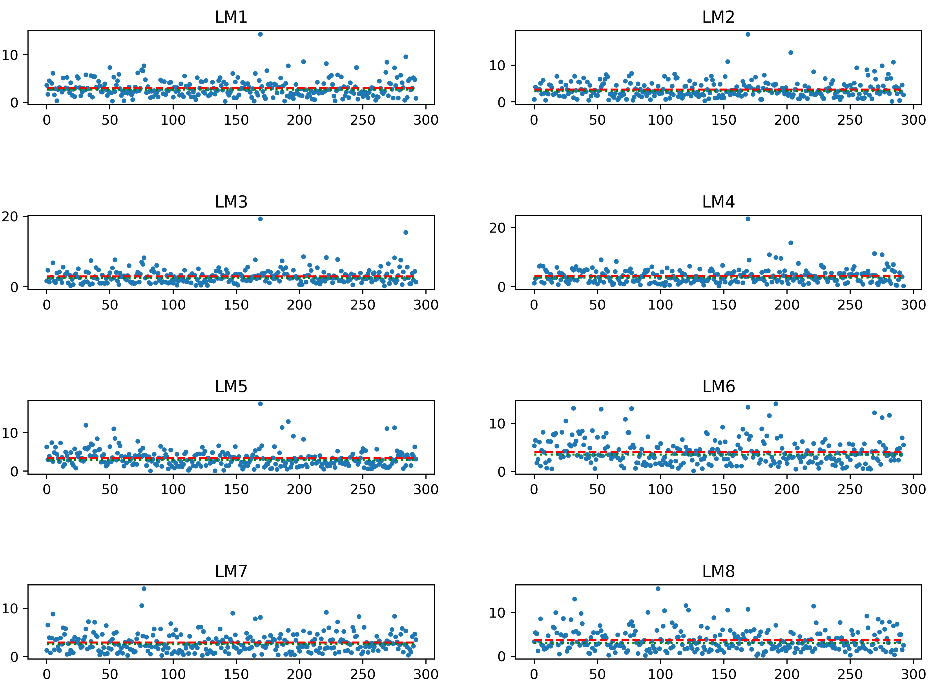
\includegraphics[scale=0.4]{images/charts/pronotum_2.png}
    \caption{The distribution of distances on each landmark on pronotum images}
\end{figure}

\begin{figure}[htbp]
    \centering
    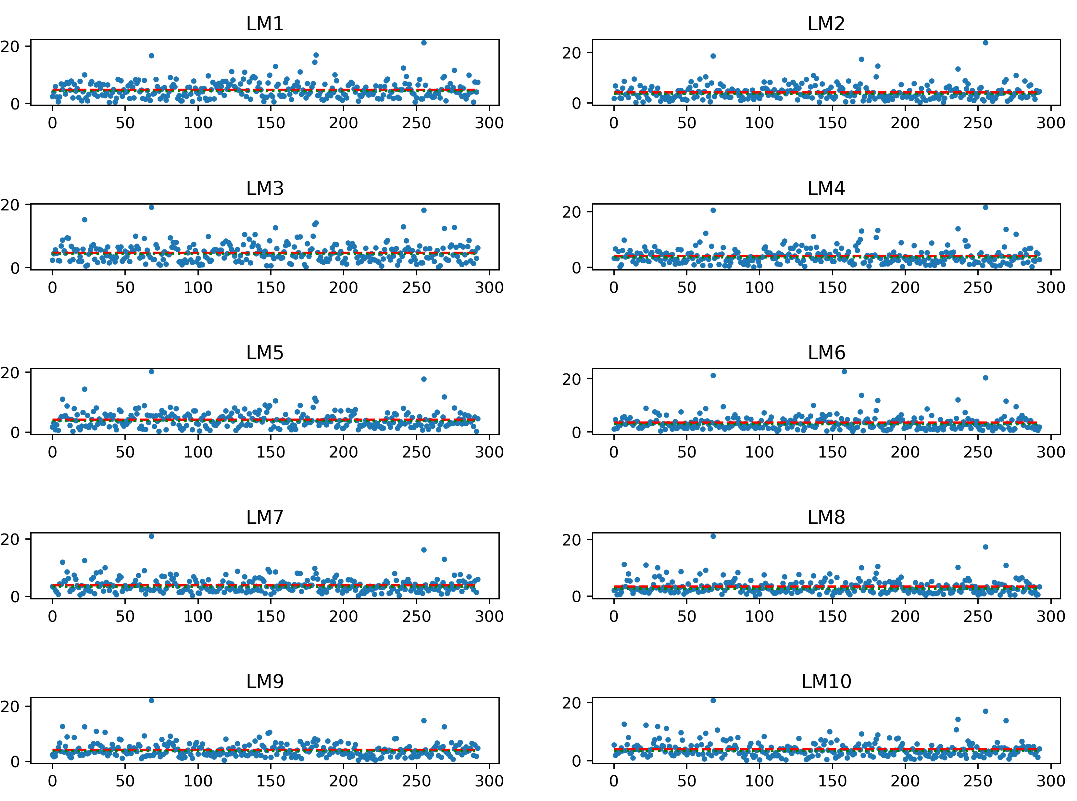
\includegraphics[scale=0.5]{images/charts/tete_2.png}
    \caption{The distribution of distances on each landmark on head images}
\end{figure}

\begin{figure}[htbp]
    \centering
    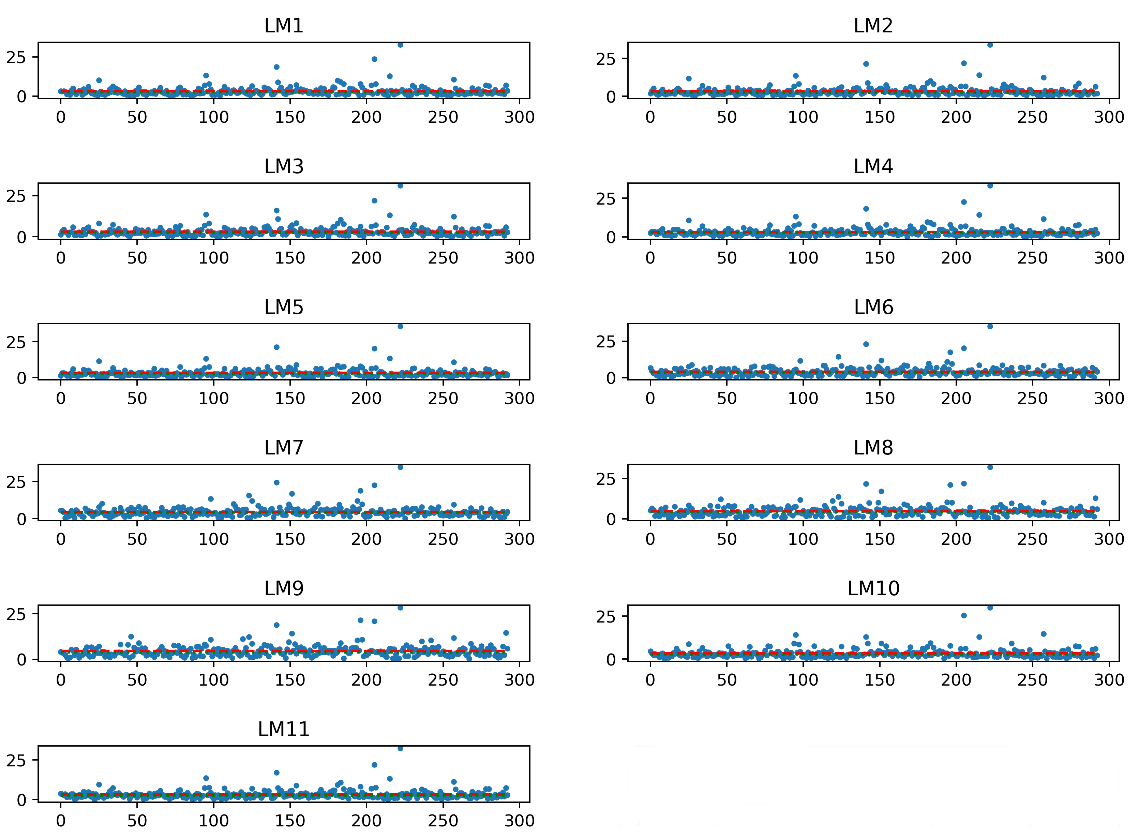
\includegraphics[scale=0.5]{images/charts/elytre_2.png}
    \caption{The distribution of distances on each landmark on elytra images}
\end{figure}

\begin{figure}[htbp]
    \centering
    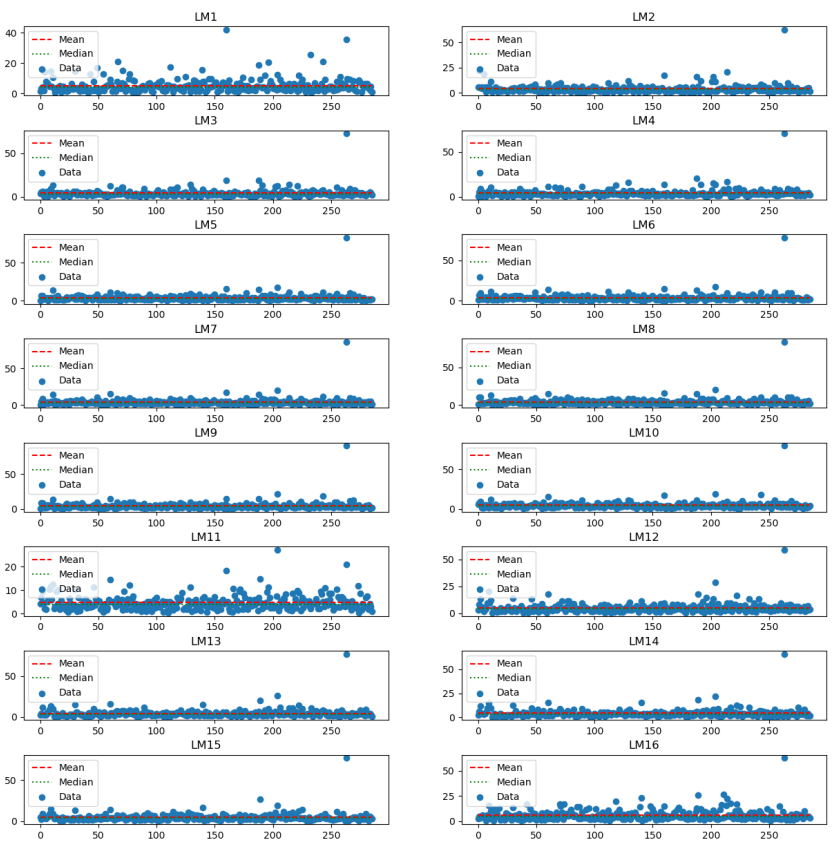
\includegraphics[scale=0.5]{images/charts/mg_2.png}
    \caption{The distribution of distances on each landmark on left mandible images}
\end{figure}

\begin{figure}[htbp]
    \centering
    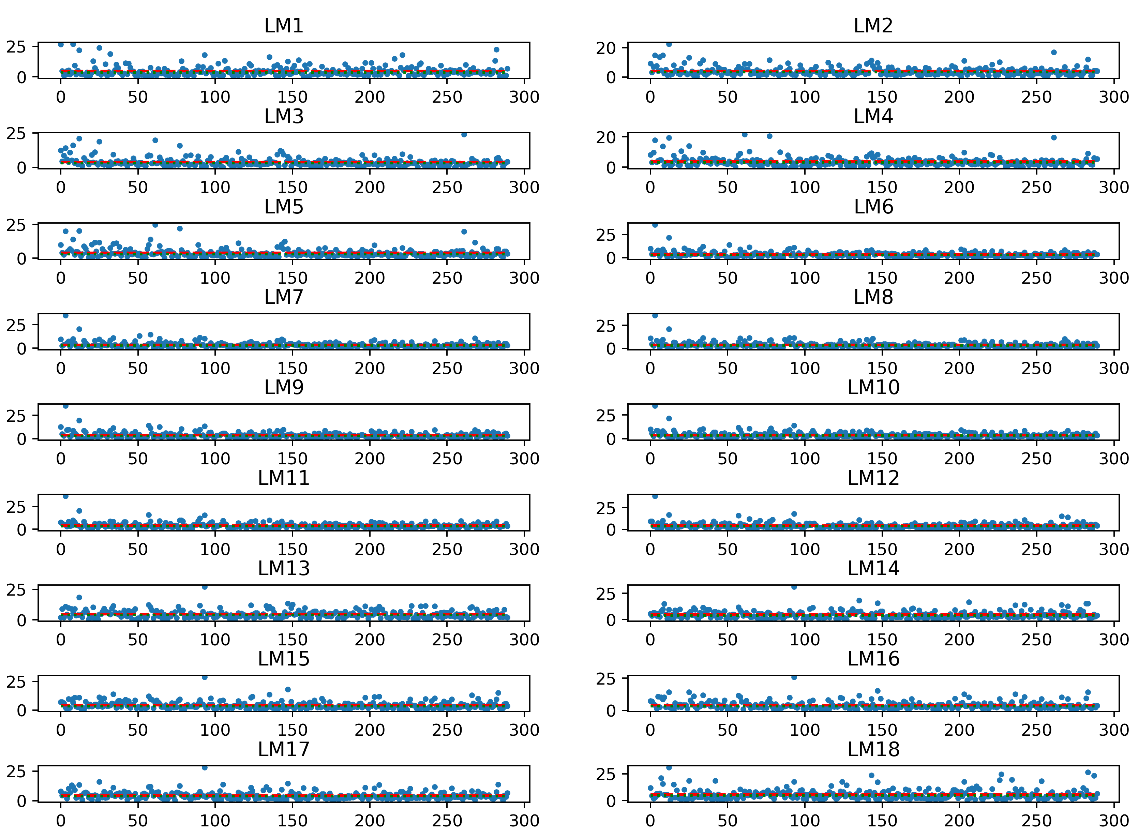
\includegraphics[scale=0.5]{images/charts/md_2.png}
    \caption{The distribution of distances on each landmark on righ mandible images}
\end{figure}
\end{document}























































Besides, the hyper-parameters (learning rate, momentum) are also kept the same as when training from scratch on each part of beelte. However, we have increased the number of epochs to $10,000$ instead of $5,000$ to achieve better learning on the parameters. The RMSE\footnote{RMSE: Root Mean Square Error} score that we have obtained is $1.1464$. This score is better than top $3$ on the leader board of challenge.
\iffalse
\begin{figure}[htbp]
    \centering
    %\subfloat[Head]{\label{}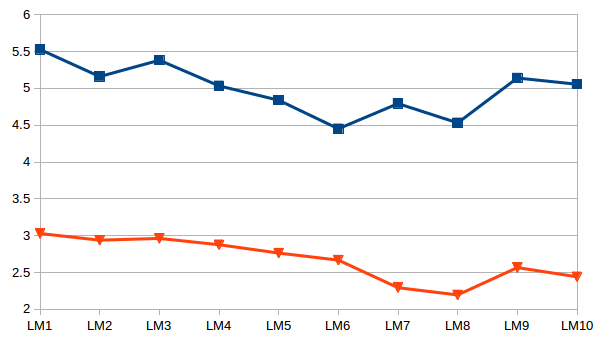
\includegraphics[width=0.5\textwidth]{images/tete_part}}~~
	%\subfloat[Elytra]{\label{}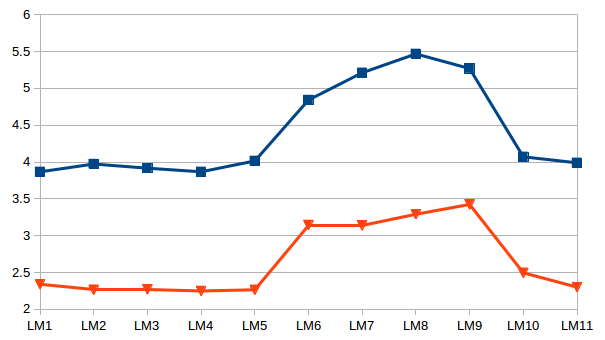
\includegraphics[width=0.5\textwidth]{images/elytre_part}}\\
	\subfloat[Pronotum]{\label{}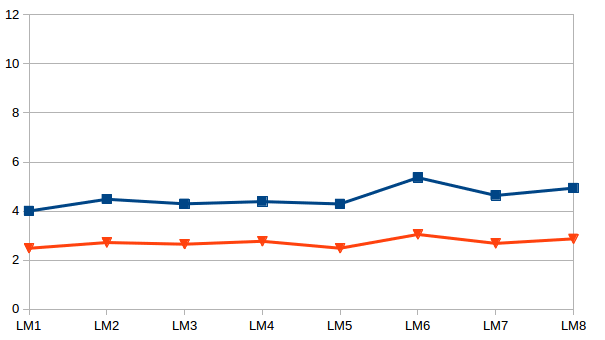
\includegraphics[width=0.5\textwidth]{images/pronotum_part.png}}
    \caption{The distribution of average distances on each landmark of pronotum part. Blue and orange lines present for the results when train the model from scratch and apply fine-tuning, respectively. }
    \label{figdist5parts}
\end{figure}
\fi
In another view, Fig. \ref{figdistmans} shows the comparison of the average distance distributions on pronotum, left and right mandible dataset. The \textbf{blue} curves present for the average distances on each landmarks when we train the model from scratch, \textbf{orange} curve present the results using fine-tuning process. In the case of $2$ mandibles (left and right), we have previously predicted landmarks with a set of image processing methods (hough transform, PCAI \cite{le2017maelab}), the black curves (Fig. \ref{figdistmans}) present these results in order to appreciate them. It is worth to remind that this method requires a segmentation step which has not been ``applicable" on the other parts. Comparing with the image processing procedure, the results are not the same between left and right mandibles, the results on the left mandible have been improved. Moreover, the results from deep learning processes are more stable for all landmarks than image processing procedures. 

Addition, in the cases of pronotum and head part, even if we plus the average distance and its standard deviation, the results are also less than the result when we trained the model from scratch.

The combined dataset then used to train the third architecture with $16$ outputs ($8$ landmarks). Then, the trained model is used to fine-tuning on each dataset. To compare the result with the previous one, we have also fine-tuned the trained model with different dataset by applying cross-validation. Firstly, we consider the losses during fine-tuning. \textit{For example}, Table. \ref{tblftpronotum}, \ref{tblftbody}, \ref{tblfthead} show the losses during fine-tuning on pronotum, elytra, and head dataset, respectively. Comparing with the losses when we trained the model from scratch, \textit{i.e.} on pronotum, the validation losses of all round in this scenario have been significantly decreased (around $40\%$).

On each part, the landmarks are predicted on the test images. Then, the average error based on the distances between predicted and corresponding manual landmarks have been also computed. Tables. \ref{tblcmppronotum}, \ref{tblcmpbody}, \ref{tblcmphead}, \ref{tblcmpmg}, and \ref{tblcmpmd} show the average distances per landmark on pronotum, elytra, head, left and right mandibles dataset, respectively. \textbf{From scratch} columns remind the previously average distances. \textbf{Fine-tune} columns present the new average distances after applying fine-tuning on each part. It is clearly shown that the result of predicted landmarks with the help of fine-tuning is more precise than training from scratch. The average distance at each landmark has decreased. Additional, when comparing the average distances between two processes, the worse case of fine-tuning process is still better than the best case of training from scratch.

\begin{table}[htbp]
	\begin{minipage}[t]{0.45\textwidth}
	\centering
	\begin{tabular}{l p{1.5cm} p{1.5cm}}
	Round & Training loss & Validation loss \\ \hline
	1 & 0.00019 & 0.00009  \\ \hline
	2 & 0.00018 & 0.00010 \\ \hline
	3 & 0.00018 & 0.00010 \\ \hline
	4 & 0.00019 & 0.00008 \\ \hline
	5 & 0.00019 & 0.00009 \\ \hline
	6 & 0.00018 & 0.00008 \\ \hline
	7 & 0.00019 & 0.00008 \\ \hline
	8 & 0.00018 & 0.00006 \\ \hline
	9 & 0.00018 & 0.00009 \\ \hline
	\end{tabular}
	\caption{The losses during fine-tuning model on pronotum dataset}
	\label{tblftpronotum}
\end{minipage}
\hfill
\begin{minipage}[t]{0.45\textwidth}
\centering
\begin{tabular}{|c|c|c|}
\hline
\textbf{$\#$LM} & \textbf{From scratch} & \textbf{Fine-tune} \\ \hline
1 & \textcolor{green}{\textbf{4.00 }}& \textcolor{green}{\textbf{2.49}}  \\ \hline
2 & 4.48 & 2.72  \\ \hline
3 & 4.30  & 2.65 \\ \hline
4 & 4.39  & 2.77 \\ \hline
5 & 4.29  & \textcolor{green}{\textbf{2.49}} \\ \hline
6 & \textcolor{red}{\textbf{5.36}}  & \textcolor{red}{\textbf{3.05}} \\ \hline
7 & 4.64  & 2.68 \\ \hline
8 & 4.94  & 2.87 \\ \hline
\end{tabular}
\caption{The average error distances per landmark of two deep learning processes on pronotum images}
\label{tblcmppronotum}
\end{minipage}
\end{table}

\begin{table}[htbp]
	\begin{minipage}[t]{0.45\textwidth}
	\centering
	\begin{tabular}{c p{1.5cm} p{1.5cm}}
	Round & Training loss & Validation loss \\ \hline
	1 & 0.00020 & 0.00006  \\ \hline
	2 & 0.00020 & 0.00006 \\ \hline
	3 & 0.00021 & 0.00006 \\ \hline
	4 & 0.00021 & 0.00006 \\ \hline
	5 & 0.00019 & 0.00006 \\ \hline
	6 & 0.00019 & 0.00006 \\ \hline
	7 & 0.00018 & 0.00005 \\ \hline
	8 & 0.00020 & 0.00006 \\ \hline
	9 & 0.00019 & 0.00006 \\ \hline
	\end{tabular}
	\caption{The losses during fine-tuning model on elytra dataset}
	\label{tblftbody}
\end{minipage}
\hfill
\begin{minipage}[t]{0.45\textwidth}
\centering
\begin{tabular}{|c|c|c|}
\hline
\textbf{$\#$LM} & \textbf{From scratch} & \textbf{Fine-tune} \\ \hline
\textbf{1} & \textcolor{green}{\textbf{3.87}} & 2.34  \\ \hline
2 & 3.97 & 2.27  \\ \hline
3 & 3.92  & 2.27 \\ \hline
4 & \textcolor{green}{\textbf{3.87}}  & \textcolor{green}{\textbf{2.25}} \\ \hline
5 & 4.02  & 2.27 \\ \hline
\textbf{6} & 4.84  & 3.14 \\ \hline
7 & 5.21  & 3.14 \\ \hline
8 & \textcolor{red}{\textbf{5.47}}  & 3.29 \\ \hline
\textbf{9} & 5.27  & \textcolor{red}{\textbf{3.42}} \\ \hline
10 & 4.07  & 2.49 \\ \hline
11 & 3.99  & 2.30 \\ \hline
\end{tabular}
\caption{The average error distances per landmark of two deep learning processes on elytra images}
\label{tblcmpbody}
\end{minipage}
\end{table}

\begin{table}[htbp]
\begin{minipage}[t]{0.45\textwidth}
	\centering
	\begin{tabular}{l p{1.5cm} p{1.5cm}}
	Round & Training loss & Validation loss \\ \hline
	1 & 0.00022 & 0.00007  \\ \hline
	2 & 0.00022 & 0.00007 \\ \hline
	3 & 0.00023 & 0.00008 \\ \hline
	4 & 0.00023 & 0.00008 \\ \hline
	5 & 0.00022 & 0.00008 \\ \hline
	6 & 0.00023 & 0.00007 \\ \hline
	7 & 0.00022 & 0.00008 \\ \hline
	8 & 0.00023 & 0.00007 \\ \hline
	9 & 0.00024 & 0.00008 \\ \hline
	\end{tabular}
	\caption{The losses during fine-tuning model on head dataset}
	\label{tblfthead}
\end{minipage}
\hfill
\begin{minipage}[t]{0.45\textwidth}
\centering
\begin{tabular}{|c|c|c|}
\hline
\textbf{$\#$LM} & \textbf{From scratch} & \textbf{Fine-tune} \\ \hline
1 & \textcolor{red}{\textbf{5.53}} & \textcolor{red}{\textbf{3.03}}  \\ \hline
2 & 5.16 & 2.94  \\ \hline
3 & 5.38  & 2.96 \\ \hline
4 & 5.03  & 2.88 \\ \hline
\textbf{5} & 4.84  & 2.76 \\ \hline
\textbf{6} & \textcolor{green}{\textbf{4.45}}  & 2.67 \\ \hline
7 & 4.79  & 2.29 \\ \hline
8 & 4.53  & \textcolor{green}{\textbf{2.20}} \\ \hline
9 & 5.14  & 2.57 \\ \hline
10 & 5.06  & 2.44 \\ \hline
\end{tabular}
\caption{The average error distances per landmark of two deep learning processes on head images}
\label{tblcmphead}
\end{minipage}
\end{table}

\begin{table}[htbp]
\begin{minipage}[t]{0.45\textwidth}
\centering
\begin{tabular}{|c|c|c|}
		\hline
		\textbf{$\#$LM} & \textbf{From scratch} & \textbf{Fine-tune} \\ \hline
		1 & \textcolor{red}{\textbf{9.1267}} & \textcolor{red}{\textbf{6.7655}} \\ \hline
		2 & \textcolor{green}{\textbf{6.7198}} & \textcolor{green}{\textbf{5.2952}} \\ \hline
		3 & 6.8704 & 5.3468 \\ \hline
		4 & 6.7719 & 5.332 \\ \hline
		5 & 7.125 & 5.4391 \\ \hline
		6 & 6.9441 & 5.3004 \\ \hline
		7 & 7.3158 & 5.5314 \\ \hline
		8 & 7.4142 & 5.6486 \\ \hline
		9 & 7.5846 & 5.8864 \\ \hline
		10 & 7.6349 & 5.9245 \\ \hline
		11 & 7.6873 & 5.972 \\ \hline
		12 & 8.4248 & 6.5755 \\ \hline
		13 & 7.9983 & 6.1067 \\ \hline
		14 & 7.4919 & 5.6307 \\ \hline
		15 & 7.7903 & 5.8522 \\ \hline
		16 & 8.5198 & 7.174 \\ \hline
	\end{tabular}
\caption{The average error distances per landmark of two deep learning processes on left mandible images}
\label{tblcmpmg}
\end{minipage}
\hfill
\begin{minipage}[t]{0.45\textwidth}
\centering
\begin{tabular}{|c|c|c|}
\hline
\textbf{$\#$LM} & \textbf{From scratch} & \textbf{Fine-tune} \\ \hline
		1 & \textcolor{red}{\textbf{9.4981}} & 6.3236 \\ \hline
	2 & 7.1657 & 5.1347 \\ \hline
	3 & 7.242 & 5.1613 \\ \hline
	4 & \textcolor{green}{\textbf{7.0436}} & \textcolor{green}{\textbf{5.0537}} \\ \hline
	5 & 7.1599 & 5.1372 \\ \hline
	6 & 7.5699 & 5.301 \\ \hline
	7 & 7.4251 & 5.2064 \\ \hline
	8 & 7.6636 & 5.5168 \\ \hline
	9 & 7.7906 & 5.6858 \\ \hline
	10 & 8.0197 & 5.7495 \\ \hline
	11 & 8.314 & 6.1975 \\ \hline
	12 & 8.1564 & 6.1898 \\ \hline
	13 & 8.8879 & 6.7612 \\ \hline
	14 & 9.1842 & \textcolor{red}{\textbf{7.0694}} \\ \hline
	15 & 8.7875 & 6.5293 \\ \hline
	16 & 8.3141 & 6.1147 \\ \hline
	17 & 8.2866 & 6.2881 \\ \hline
	18 & 8.8928 & 6.8367 \\ \hline
\end{tabular}
\caption{The average error distances per landmark of two deep learning processes on right mandible images}
\label{tblcmpmd}
\end{minipage}
\end{table}






\begin{table}[htbp]
\begin{minipage}{0.5\linewidth}
	\centering
	\begin{tabular}{|c|c|}
		\hline
		\textbf{Landmark} & \textbf{Distance} (in pixels) \\ \hline
		1 & 3.8669  \\ \hline
		2 & 3.9730 \\ \hline
		3 & 3.9166 \\ \hline
		4 & 3.8673 \\ \hline
		5 & 4.0151 \\ \hline
		6 & 4.8426 \\ \hline
		7 & 5.2125 \\ \hline
		8 & 5.4685 \\ \hline
		9 & 5.2692 \\ \hline
		10 & 4.0709 \\ \hline
		11 & 3.9896 \\ \hline
	\end{tabular}
	\caption{\small{The average distance on all images per landmark on \textbf{elytra} images}}
	\label{tblavgdiselytra}
\end{minipage}
\hfill
\begin{minipage}{0.5\linewidth}
	\centering
	\begin{tabular}{|c|c|}
		\hline
		\textbf{Landmark} & \textbf{Distance} (in pixels) \\ \hline
		1 & 5.5280  \\ \hline
		2 & 5.1609 \\ \hline
		3 & 5.3827 \\ \hline
		4 & 5.0345 \\ \hline
		5 & 4.8393 \\ \hline
		6 & 4.4516 \\ \hline
		7 & 4.7937 \\ \hline
		8 & 4.5322 \\ \hline
		9 & 5.1412 \\ \hline
		10 & 5.0564 \\ \hline
	\end{tabular}
	\caption{\small{The average distance on all images per landmark on \textbf{head} images}}
	\label{tblavgdishead}
\end{minipage}
\end{table}

\begin{table}[htbp]
\begin{minipage}{0.5\linewidth}
	\centering
	\begin{tabular}{|c|c|}
		\hline
		\textbf{Landmark} & \textbf{Distance} (in pixels) \\ \hline
		1 & 9.1267  \\ \hline
		2 & 6.7198 \\ \hline
		3 & 6.8704 \\ \hline
		4 & 6.7719 \\ \hline
		5 & 7.1250 \\ \hline
		6 & 6.9441 \\ \hline
		7 & 7.3158 \\ \hline
		8 & 7.4142 \\ \hline
		9 & 7.5846 \\ \hline
		10 & 7.6349 \\ \hline
		11 & 7.6873 \\ \hline
		12 & 8.4248 \\ \hline
		13 & 7.9983 \\ \hline
		14 & 7.4919 \\ \hline
		15 & 7.7903 \\ \hline
		16 & 8.5198 \\ \hline
	\end{tabular}
	\caption{\small{The average distance on all images per landmark on \textbf{left mandible} images}}
	\label{tblavgdislmandible}
\end{minipage}
\hfill
\begin{minipage}{0.5\linewidth}
	\centering
	\begin{tabular}{|c|c|}
		\hline
		\textbf{Landmark} & \textbf{Distance} (in pixels) \\ \hline
		1 & 9.4981  \\ \hline
		2 & 7.1657 \\ \hline
		3 & 7.2420 \\ \hline
		4 & 7.0436 \\ \hline
		5 & 7.1599 \\ \hline
		6 & 7.5699 \\ \hline
		7 & 7.4251 \\ \hline
		8 & 7.6636 \\ \hline
		9 & 7.7906 \\ \hline
		10 & 8.0197 \\ \hline
		11 & 8.3140 \\ \hline
		12 & 8.1564 \\ \hline
		13 & 8.8879 \\ \hline
		14 & 9.1842 \\ \hline
		15 & 8.7875 \\ \hline
		16 & 8.3141 \\ \hline
		17 & 8.2866 \\ \hline
		18 & 8.8928 \\ \hline
	\end{tabular}
	\caption{\small{The average distance on all images per landmark on \textbf{right mandible} images}}
	\label{tblavgdisrmandible}
\end{minipage}
\end{table}
In geometric morphometry, landmarks (or points of interest) are important features to describe the shape. Depending on the complicacy of the objects in the image, setting automatic landmarks can rely on different methods. When the object can be segmented, the image processing techniques may applied to predict the landmarks. Lowe et al. \cite{lowe2004distinctive} have proposed SIFT method to identify the keypoints on 2D images by extracting the distinctive features from the images. It is composed by four steps: (1) scale space extrema detection: a difference of Gaussian (DoG) function is applied to identify the interested points at all scales; (2) keypoint localization: the keypoint candidates are localized and refined by deleting the points which have the low contrast or not localized along the edge; (3) orientation assigment: for each keypoint candidates, the orientation and gradient magnitude are computed by considering their 4-neighborhoods; (4) keypoint descriptor are computed for each keypoint from its orientation and gradient magnitude. From the descriptors of the keypoints, they can be used to find the corresponding points between two images. SURF is another method which has been proposed by Herbert Bay et al. \cite{bay2006surf}. The SURF algorithm is the same principles with SIFT but details in each step are different. This algorithm mainly has three steps: (1) keypoints detection, (2) local neighborhood description and (3) matching. Different with SIFT, SURF uses a blob detector base on the Hessian matrix to find the keypoints. The Hessian matrix is used as a measure of local change around the point and chooses the points where this determinant is maximal. Then, the descriptors are computed around the key points by describing the intensity distribution of keypoint's neighborhoods. The matching points from different images are obtained by comparing the descriptors of the key points. Palaniswamy et al. \cite{palaniswamy2010automatic} have proposed a method to automatically detect the landmarks on 2D images of Drosophila wings (Fig. \ref{imgflywing}). The method is mainly based on probabilistic Hough Transform. It includes four steps: (1) features detection of the fly wing structure (segmentation); (2) using pairwise geometric histogram (PGH) to record the compact invariant shape descriptor; (3) estimating the global pose of wing using the probabilistic Hough transform; (4) and finally a template matching is applied to refine the correctly of individual features.

\begin{figure}
	\centering
	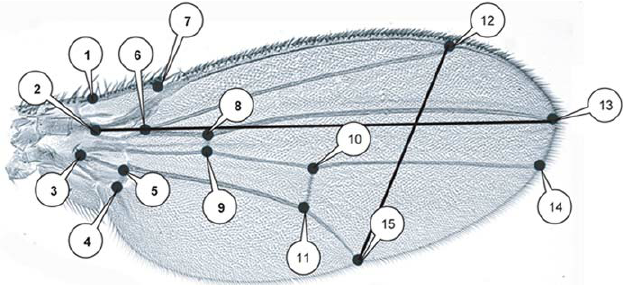
\includegraphics[scale=.4]{images/wing_landmarks}	
	\caption{A Drosophila wing and its landmarks}
	\label{imgflywing}
\end{figure}

To illustrate the final results, we display the distribution of
the distances in both cases: the best and the worst results (resp. landmark $1$ and $6$ on pronotum dataset) of five datasets (pronotum, elytra, head, left and right mandible) in  
Fig. \ref{figdist3parts}, \ref{figdist3partselytre}, \ref{figdist3partstete}, \ref{figdist3partsmg}, and \ref{figdist3partsmd}, respectively. In these figures, the left images present for the results when we trained the model from scratch; while the right images shows the results after applying fine-tuning. The blue lines in the charts present the average distance values. Clearly, the results in the fine-tuning case have been improved significantly than training from scratch.

\begin{figure}[htbp]
    \centering
    \subfloat[Landmark 1 - CNN]{\label{figdist3parts1}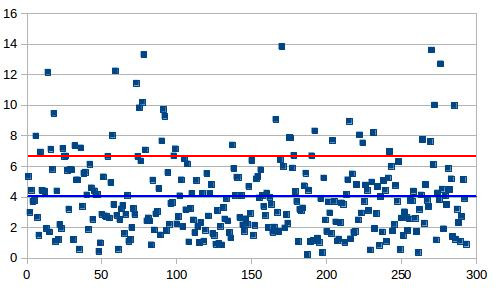
\includegraphics[width=0.5\textwidth]{images/lm1_cnn_2}}~~
	\subfloat[Landmark 1 - fine-tuning]{\label{figdist3parts2}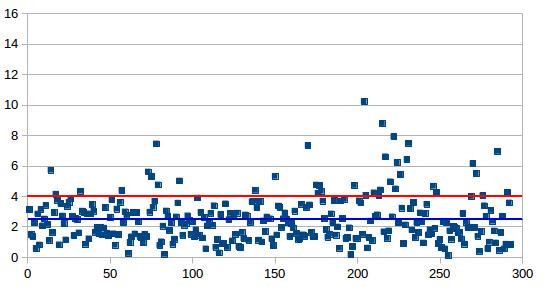
\includegraphics[width=0.5\textwidth]{images/lm1_finetuning_2}}\\
	\subfloat[Landmark 6 - CNN]{\label{figdist3parts3}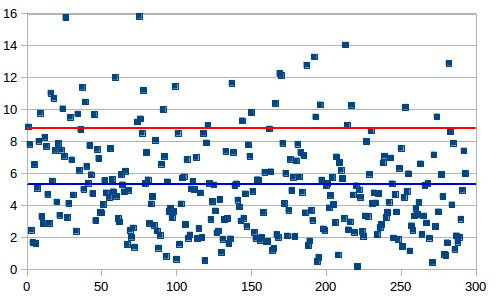
\includegraphics[width=0.5\textwidth]{images/lm6_cnn_2}}~~
	\subfloat[Landmark 6 - fine-tuning]{\label{figdist3parts4}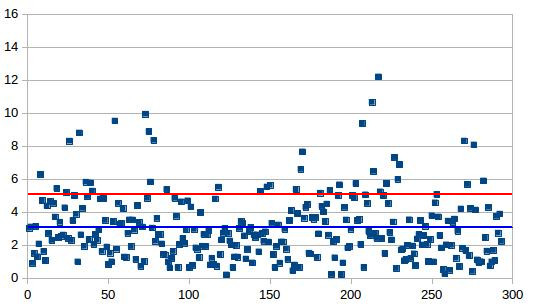
\includegraphics[width=0.5\textwidth]{images/lm6_finetuning_2}}\\
    \caption{The distribution of distances on $1^{st}$ and $6^{th}$
landmarks of all images in two testing steps (CNN and fine-tuning) (on \textbf{pronotum} dataset). The red line presents the standard deviation value.}
    \label{figdist3parts}
\end{figure}

\begin{figure}[htbp]
    \centering
    \subfloat[Landmark 1 - CNN]{\label{figdist3partselytre1}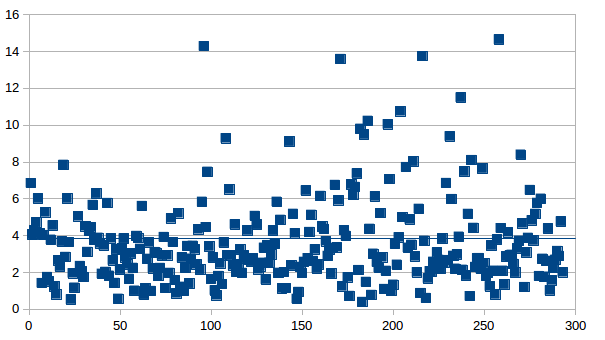
\includegraphics[width=0.4\textwidth]{images/fsc_elytre_lm1}}~~
	\subfloat[Landmark 1 - fine-tuning]{\label{figdist3partselytre2}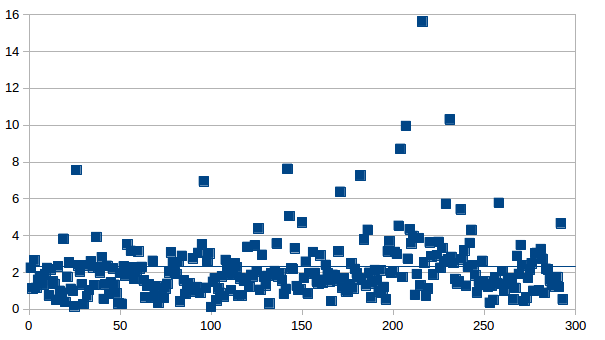
\includegraphics[width=0.4\textwidth]{images/fn_elytre_lm1}}\\
	\subfloat[Landmark 8 - CNN]{\label{figdist3partselytre3}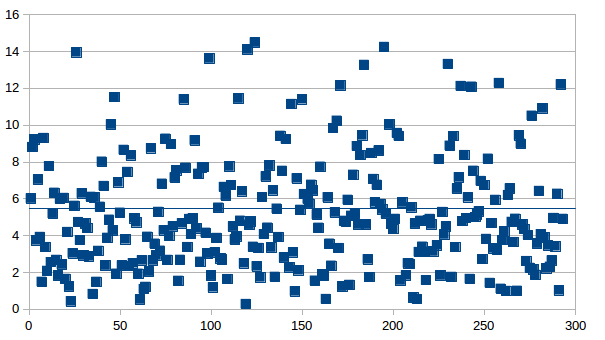
\includegraphics[width=0.4\textwidth]{images/fsc_elytre_lm8}}~~
	\subfloat[Landmark 8 - fine-tuning]{\label{figdist3partselytre4}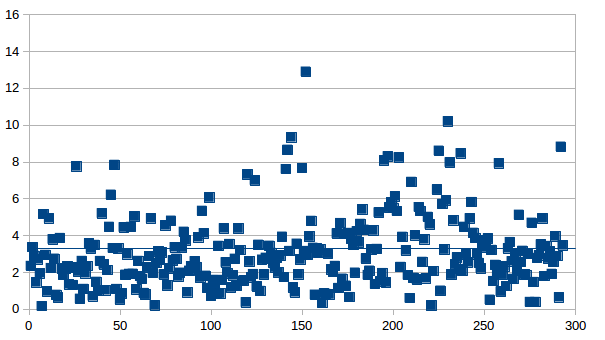
\includegraphics[width=0.4\textwidth]{images/fn_elytre_lm8}}\\
    \caption{The distribution of distances on $1^{st}$ and $8^{th}$
landmarks of all images in two testing steps (CNN and fine-tuning) (on \textbf{elytra} dataset).}
    \label{figdist3partselytre}
\end{figure}

\begin{figure}[htbp]
    \centering
    \subfloat[Landmark 1 - CNN]{\label{figdist3partstete1}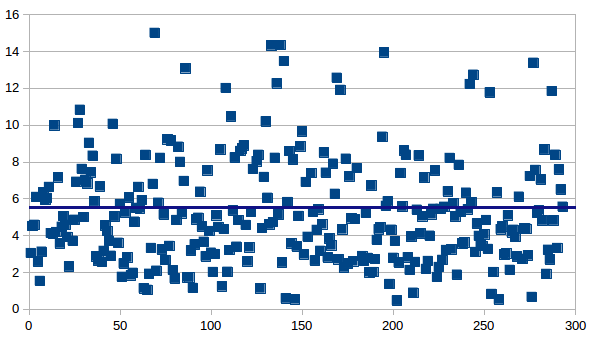
\includegraphics[width=0.4\textwidth]{images/fsc_tete_lm1}}~~
	\subfloat[Landmark 1 - fine-tuning]{\label{figdist3partstete2}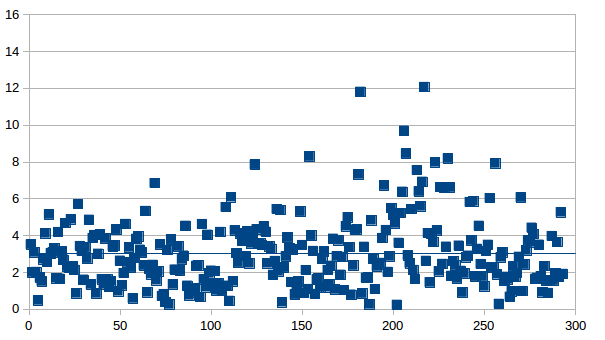
\includegraphics[width=0.4\textwidth]{images/fn_tete_lm1}}\\
	\subfloat[Landmark 6 - CNN]{\label{figdist3partstete3}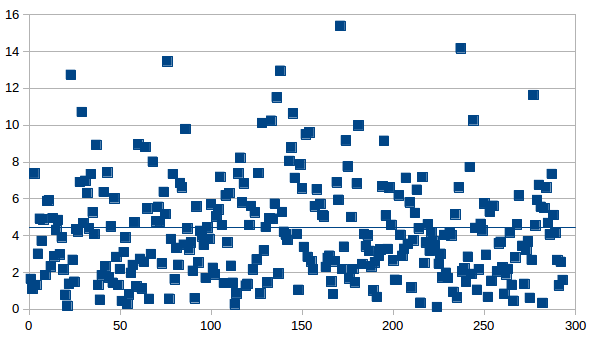
\includegraphics[width=0.4\textwidth]{images/fsc_tete_lm6}}~~
	\subfloat[Landmark 6 - fine-tuning]{\label{figdist3partstete4}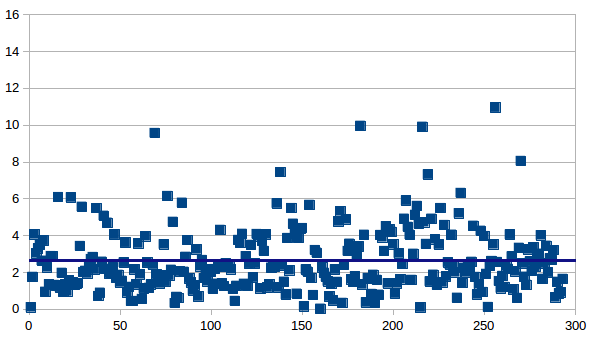
\includegraphics[width=0.4\textwidth]{images/fn_tete_lm6}}\\
    \caption{The distribution of distances on $1^{st}$ and $6^{th}$
landmarks of all images in two testing steps (CNN and fine-tuning) (on \textbf{head} dataset).}
    \label{figdist3partstete}
\end{figure}

\begin{figure}[htbp]
    \centering
    \subfloat[Landmark 4 - CNN]{\label{figdist3partstete1}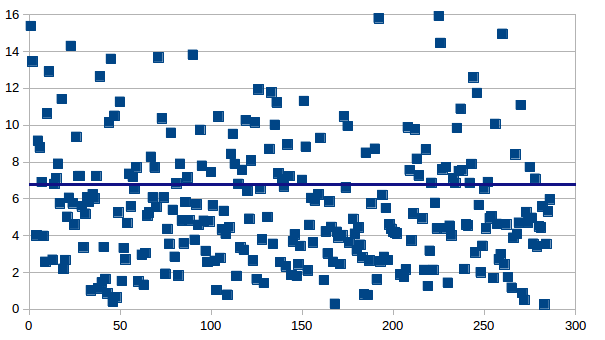
\includegraphics[width=0.4\textwidth]{images/fsc_mg_lm4}}~~
	\subfloat[Landmark 4 - fine-tuning]{\label{figdist3partstete2}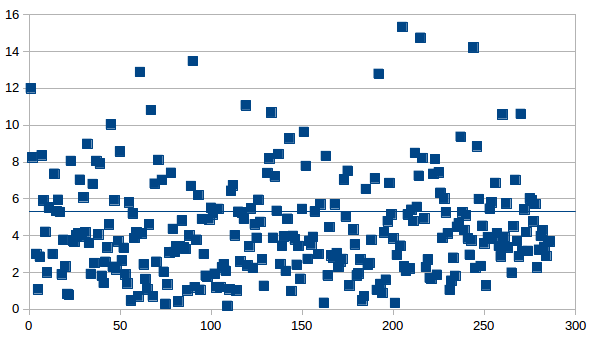
\includegraphics[width=0.4\textwidth]{images/fn_mg_lm4}}\\
	\subfloat[Landmark 1 - CNN]{\label{figdist3partstete3}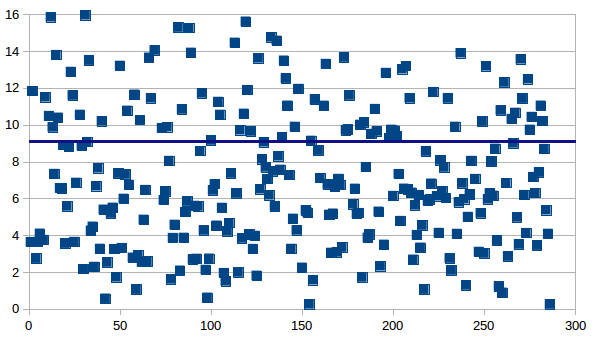
\includegraphics[width=0.4\textwidth]{images/fsc_mg_lm1}}~~
	\subfloat[Landmark 1 - fine-tuning]{\label{figdist3partstete4}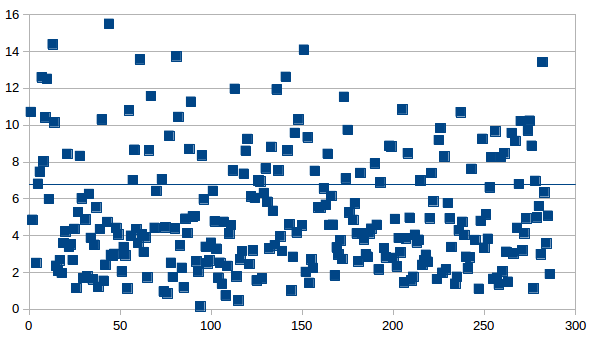
\includegraphics[width=0.4\textwidth]{images/fn_mg_lm1}}\\
    \caption{The distribution of distances on $1^{st}$ and $4^{th}$
landmarks of all images in two testing steps (CNN and fine-tuning) (on \textbf{left mandible} dataset).}
    \label{figdist3partsmg}
\end{figure}

\begin{figure}[htbp]
    \centering
    \subfloat[Landmark 4 - CNN]{\label{figdist3partstete1}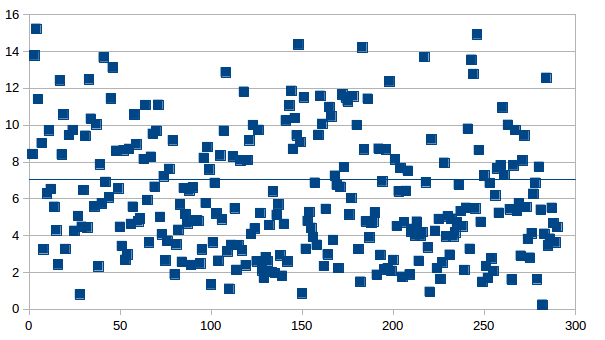
\includegraphics[width=0.4\textwidth]{images/fsc_md_lm4}}~~
	\subfloat[Landmark 4 - fine-tuning]{\label{figdist3partstete2}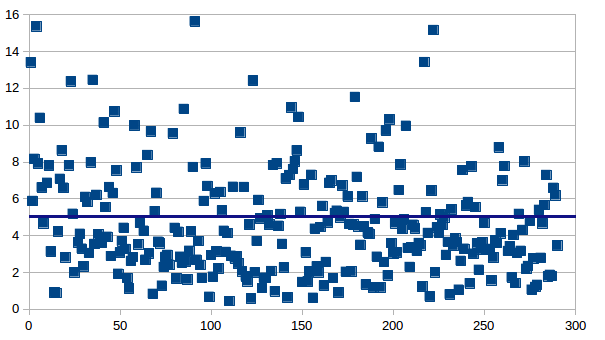
\includegraphics[width=0.4\textwidth]{images/fn_md_lm4}}\\
	\subfloat[Landmark 1 - CNN]{\label{figdist3partstete3}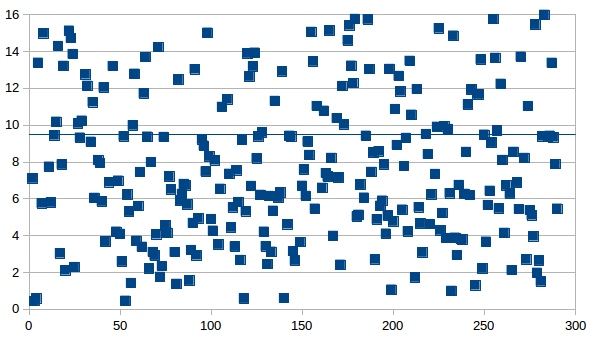
\includegraphics[width=0.4\textwidth]{images/fsc_md_lm1}}~~
	\subfloat[Landmark 1 - fine-tuning]{\label{figdist3partstete4}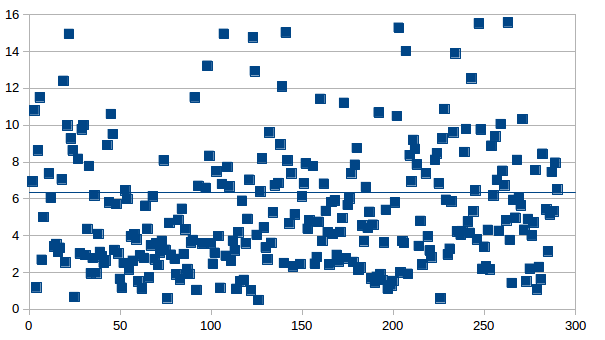
\includegraphics[width=0.4\textwidth]{images/fn_md_lm1}}\\
    \caption{The distribution of distances on $1^{st}$ and $4^{th}$
landmarks of all images in two testing steps (CNN and fine-tuning) (on \textbf{right mandible} dataset).}
    \label{figdist3partsmd}
\end{figure}

% Introduction
 A CNN consists of an input, an output layer, as well as one or multiple hidden layers. An input after being put on the network will be passed through a series of hidden layers before giving the outputs at the last layer. The computing of CNN affects on $3$ dimensions of data: width, height, and depth. 
 
 % model 2
 
The second architecture is modified from the first model. The layers are kept the same as the first one but the outputs of the first of two FC layers are changed from $500$ (in the first model) to $1000$ (Fig. \ref{fignet2}). Increasing the value at FC layers is hoping to obtain more features from CONV layer to give the decision without requirements of a lot of new capacity resources. However, the obtained results have not been satisfying, it will be discussed in the last section (Section \ref{sexperiments}). 

\begin{figure}[h]
	\centering
	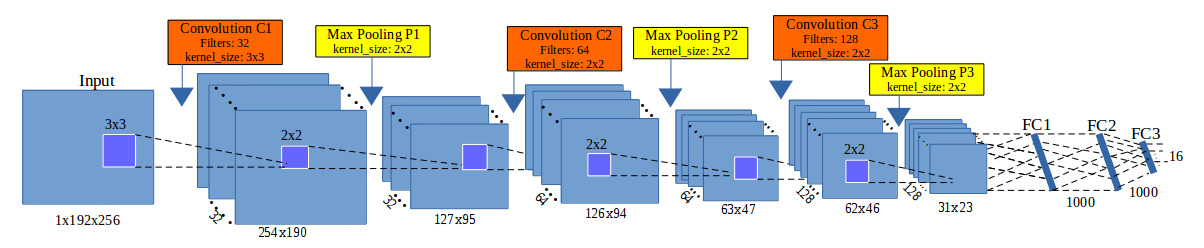
\includegraphics[scale=0.3]{images/net2}
	\caption{The architecture of the second model}
	\label{fignet2}
\end{figure}
%Clearly, the deeper models have provided better results but it also increases the complexity of the network, which makes the network be more difficult to optimize and easy to get overfitting.
%Deep learning \cite{lecun2015deep} has been introduced in the middle of the previous century for artificial intelligence application but it has encountered several problems to take real-world cases such as memory or computing time. Luckily, the improvements of computing capacities, both in memory size and in computing time with GPU programming, have opened new perspective for deep learning. In recent years, deep learning architectures are known as the solutions for the tasks in computer vision. Especially in image analysis, CNNs, which consist of convolutional layers, pooling layers, full connected layers, are used to solve the classification or recognition tasks. For example, LeNet \cite{lecun1998gradient} has been known as the first architecture of CNN to read the zip codes and digits. It had a standard structure stacked convolutional layers (normalization and max-pooling) are followed by one or more full-connected layers. From this architecture, many models have been proposed to improve the accuracy as well as computing times in recent years. That must be mentioned to AlexNet \cite{krizhevsky2012imagenet}, ZFNet \cite{zeiler2014visualizing}, GoogLeNet \cite{szegedy2015going}, VGGNet \cite{simonyan2014very}, or ResNet \cite{he2016deep}. Besides, deep learning has been obtained the achievement in other domains such as \textbf{image recognition} \cite{szegedy2015going,farabet2013learning,li2015convolutional}, \textbf{speech recognition} \cite{mikolov2011strategies, hinton2012deep}, \textbf{language translation} \cite{jean2014using, sutskever2014sequence}, \textbf{natural language processing} \cite{lecun2015deep, collobert2011natural, collobert2008unified}, \ldots.

%For example, in \textbf{image classification}, Yann LeCun et al. \cite{lecun1998gradient} have proposed an architecture named LeNet to read the zip codes, digits, \ldots which had a standard structure stacked convolutional layers (normalization and max-pooling) are followed by one or more full-connected layers. In 2012, Alext Krizhevsky et al \cite{krizhevsky2012imagenet} proposed AlexNet, which similars to LeNet but more deeper and bigger, to classify the images into different categories. It was submitted to the ImageNet challenge and significantly outperformed the second runner-up. Ciresan et al. \cite{ciregan2012multi} proposed a multi-column deep CNNs which combining several CNNs. This network have been used for image classification and it have decreased the error rate by $30 - 40\%$. In \textbf{image recognition}, C.Szegedy et al. \cite{szegedy2015going} proposed Inception to achieve for classification and object detection, C. Farabet et al. \cite{farabet2013learning} have introduced a network to learn the hierarchical features of the images; H. Li et al. \cite{li2015convolutional} have present a CNN for detecting the human face at multiple resolutions. 

%For each beetle, the biologists have taken images of five parts: \textit{left and right mandibles, head, elytra, and pronotum} (Fig. \ref{figbeetles}). All the images are presented in the RGB color model with two dimensions. Along with each image, a set of landmarks has been marked by experts which can be used as ground truth to evaluate the predicted landmarks. During the experiments, the proposed network has been trained on the dataset by applying two strategies. In the first strategy, the network is trained from scratch on each dataset; while in the second strategy, the training process has been modified to include a fine-tuning \cite{yosinski2014transferable} stage. Besides, the value of Root Mean Square Error (RMSE) is used to compute the losses during two experiment processes.

%In some cases, the interested object is easy to extract and can be analyzed by applying the well-known image analysis procedures. Nevertheless, we can not apply the same procedure for un-segmentable images. It really becomes a challenge on the complex images. Luckily, the appearance of deep learning has seen huge success in handwritten digit recognition, speech, images classification and detecting objects in images. Now, an interesting thing is how to use deep learning for landmark detecting, which can be considered as the local characteristic of the image. Our motivation to design a CNN model that able to extract the landmarks on images (even it is segmentable or un-segmentable), which will be used to replace for the previous procedures.

%The main idea consists of the designing and training a CNN \cite{lecun2010convolutional} on a dataset with manual landmarks. Like other CNNs, the features are extracted by using a group of different layer types (i.e. convolutional layer, pooling layer,\ldots) followed by some dense layers to provide the prediction of the network. After designing, the proposed model will be trained on the dataset includes the images which are taken from $293$ beetles. For each beetle, the biologists have taken images of five parts: \textit{left and right mandibles, head, elytra, and pronotum} (Figs.\ref{figh1}, \ref{figt1}, \ref{fige1}, \ref{figlm1}, \ref{figrm1}). All the images are presented in the RGB color model with two dimensions. Along with each image, a set of landmarks has been marked by experts which can be used as ground truth to evaluate the predicted landmarks (Figs.\ref{figh2}, \ref{figt2}, \ref{fige2}, \ref{figlm2}, \ref{figrm2}). During the experiments, the proposed network has been trained on the dataset by applying two strategies. In the first strategy, the network is trained from scratch on each dataset; while in the second strategy, the training process has been modified to include a fine-tuning \cite{yosinski2014transferable} stage. Besides, the value of Root Mean Square Error (RMSE) is used to compute the losses during two experiment processes. For more information about the model, you can see at our repository on GitHub: \texttt{https://github.com/linhlevandlu/CNN\_Beetles\_Landmarks}.
\iffalse
\begin{figure}[htbp]
    \centering
    \subfloat[Head]{\label{figh1}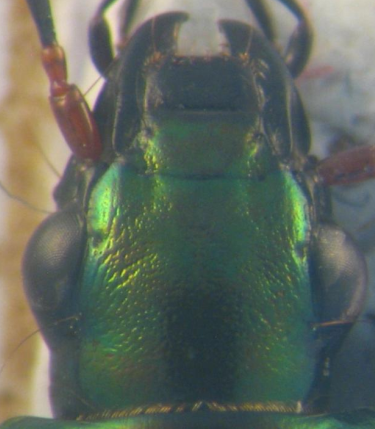
\includegraphics[width=0.3\textwidth]{images/orgHead}}~~
\subfloat[Head's manual landmarks]{\label{figh2}\includegraphics[width=0.35\textwidth]{images/lmHead}}  
    \caption{The \textbf{head} anatomical of beetle and its manual landmarks}
    \label{figbeetle1}
\end{figure}
\begin{figure}[htbp]
    \centering
\subfloat[pronotum]{\label{figt1}\includegraphics[width=0.4\textwidth]{images/orgThorax}}~~
	\subfloat[pronotum's manual landmarks]{\label{figt2}\includegraphics[width=0.4\textwidth]{images/lmThorax}}
    \caption{The \textbf{pronotum} anatomical of beetle and its manual landmarks}
    \label{figbeetle2}
\end{figure}
\begin{figure}[htbp]
    \centering
	\subfloat[Elytra]{\label{fige1}\includegraphics[width=0.3\textwidth]{images/orgElytra}}~~
\subfloat[Elytra's manual landmarks]{\label{fige2}\includegraphics[width=0.35\textwidth]{images/lmElytra}}  
    \caption{The \textbf{elytra} anatomical of beetle and its manual landmarks}
    \label{figbeetle3}
\end{figure}
\begin{figure}[htbp]
    \centering
\subfloat[Left mandible]{\label{figlm1}\includegraphics[width=0.25\textwidth]{images/orgLMandible}}~~
	\subfloat[Left mandible's manual landmarks]{\label{figlm2}\includegraphics[width=0.3\textwidth]{images/lmLMandible}}    
    \caption{The \textbf{left mandible} anatomical of beetle and its manual landmarks}
    \label{figbeetle4}
\end{figure}
\begin{figure}[htbp]
    \centering
\subfloat[Right mandible]{\label{figrm1}\includegraphics[width=0.25\textwidth]{images/orgRMandible}}~~
	\subfloat[Right mandible's manual landmarks]{\label{figrm2}\includegraphics[width=0.33\textwidth]{images/lmRMandible}}    
    \caption{The \textbf{right mandible} anatomical of beetle and its manual landmarks}
    \label{figbeetle5}
\end{figure}
\fi
%These landmarks are used in different objectives of different domains, for example, landmarks are basic characteristics to detect the human face or human pose; in biology, the topology of the objects in an organism can be measured from the location of landmarks.

%The detected key points are then used in different objectives of different domains, for example, they are fundamental to detect the human face or human pose; in biology, the topography of the objects of an organism can be measured from the location of landmarks. The emergence of deep learning has seen success in other fields of computer vision and key points detection is also not an exception. It has been used to predict the fashion landmarks \cite{liu2016fashion}, human facial key points \cite{sun2013deep,zhang2014facial}, or ear landmarks \cite{cintas2016automatic}.
 
%Key points detection has a wide use and becomes a critical in image analysis of different domains, such as: In geosciences, the key points can be used to recognize the seabed by extracting and comparing the landmarks from sonar images at different times; or computer vision, they are fundamental to detect the human face or human pose; in biology, the topography of the objects of an organism can be measured if we have enough the number of landmarks. Landmarks, or \textit{key points}, or \textit{points of interest}, are the points on the image that store important information about the shape of the object, \textit{for example}, the left and right corners of eyes are two important points to detect the human eyes. Depending on the object, the number of landmarks may  be different, as well as their position can be defined along the outline of the object or inside the object, i.e. the landmarks on Drosophila wings \cite{drosophilaWings} are stayed on the veins of the wings, but the landmarks on human ears \cite{cintas2016automatic} can be located on the ear edge or inside the pimas of the ears.

%Early methods \cite{lowe2004distinctive,bay2006surf,palaniswamy2010automatic} mainly focused on the low level-vision of the image by applying the image processing techniques, and segmentation is most often the first and the most important step in the process. This task remains a bottleneck to compute the features of the complex image. Even if the interested object is easy to extract, the process may take a bit of time to extract the exciting features. The emergence of deep learning has seen success in other fields of computer vision and key points detection is also not an exception. It has been used to predict the fashion landmarks \cite{liu2016fashion}, human facial key points \cite{sun2013deep,zhang2014facial}, or ear landmarks \cite{cintas2016automatic}.

%Besides object classification or recognition, \textbf{key points detection} is another task in image analysis. Early methods \cite{} have been achieved good results. These methods are basically divided into two groups: the regression-based methods and template fitting methods. A regression-based method predicts landmark locations by regression using image features \cite{valstar2010facial,dantone2012real,burgos2013robust}. While a template fitting method builds a template to fit with the input image, then the landmarks are setting  \cite{cootes2001active,liu2007generic,yu2013pose}. With the comeback of deep learning, CNN has been used to predict the landmarks on 2D and it has gained better results. Yi Sun et al. \cite{sun2013deep} have proposed a cascaded CNNs to predict the facial points on the human face. Their model includes the networks which have separated into three levels of the cascade. The networks recognize the human face from the global to the local view to increasing the accuracy of predicted key points. Zhanpeng Zhang et al. \cite{zhang2014facial} proposed a \textit{Tasks-Constrained Deep Convolutional Network} to optimize facial landmarks detection. Their model detected the facial landmarks with a set of related tasks such as head pose estimation, gender classification, age estimation, or facial attribute inference. Shaoli Huang et al. \cite{huang2017coarse} introduced a coarse-fine network, which composed of several coarse detector branches, to locate the keypoints and to estimate the human pose. Cintas et al. \cite{cintas2016automatic} has introduced a network to predict the landmarks on human ears (Fig. \ref{imgears}). After training, the network has the ability to detect $45$ landmarks on human ears. 
\iffalse
\begin{figure}[!h]
	\centering
	\includegraphics[scale=.4]{images/ear_landmarks}	\
	\caption{Landmarks on human ear in study of Cintas et al. \cite{cintas2016automatic}}
	\label{imgears}
\end{figure}
\fi
 
%In the past, landmarks on biological images are carried out manually or semi-automatically by applying some image processing techniques \cite{}. When the image processing techniques applied, segmentation is the most important step and this step becomes the bottleneck of the process. When the interested object easy to segment, the process may be provided the good results. But it could be a lack with the complex images (un-segmentable images). So, a method for landmarking without the help of segmentation step is very interested in and CNN has been chosen for this objective.

%As an association with the biologist, we study to develop an automatic method for predicting the landmarks on beetle's anatomical (Figs.\ref{figh1}, \ref{figt1}, \ref{fige1}, \ref{figlm1}, \ref{figrm1}). In the past, locating landmarks on biological images is mainly using image processing techniques where the object in the image is easily to segment. For example, in a previous work \cite{le2017maelab}, we have applied a series of algorithms to detect the landmarks automatically on beetles mandibles which are considered as the easied objects to segment (with an quality enough good for our need). In that work, the landmarks have been detected by registering two segmentations of images and then, using SIFT descriptor to refine the location of predicted landmarks. After the experiment, we have obtained good enough results on mandibles. Unfortunately, we have observed that the method did not provide good results when the segmentation is not precise, i.e. on pronotum or elytra images. This is explained why we have turned the automatically landmarking into another stage without any segmentation step. Using CNN for landmarking seems that a good choice for un-segmentable images.

\section{Overview of Convolutional Neural Network}
\label{sOverview}
A CNN is a feedforward network which takes the information following one direction from the inputs to the outputs. Currently, CNNs have many different variations, but in general, it consists of convolutional and pooling layers which are stacked together to convolve and to down-sample the inputs. Then, they are followed by one or more fully connected layers to give the decision as the output of the network. 

Fig. \ref{imgcnn_network} shows a classical example of a CNN for classification problem. The network inputs directly an image to several stages of convolutional and pooling layers. Then, the representation is feed into three fully connected layers. A dropout layer is inserted after the second fully connected layer (it is represented by some blue nodes). Finally, the last fully connected layer gives the category label for the input image. This architecture could be seen as the most popular one. Now, we will describe the different types of layers.

\begin{figure}[!h]
	\centering
	\includegraphics[scale=.3]{images/cnn_network_2}
	\caption{A CNN network for classification problem}
	\label{imgcnn_network}
\end{figure}

Convolutional (CONV) layer: uses as a feature extractor by applying some learnable weights (filters) on the input images. The input image is convolved with the filters in order to compute the new feature maps; then, the convolved results are sent through a nonlinear activation before sending to the next layer. In CONV layer, the neurons are arranged into feature maps. All the neurons within a feature map have the same constraints; however, different features maps within the same CONV layer have different weights so that several features can be extracted at each location of an input image. This step is similar to apply a filter operation in image processing.

Pooling (POOL) layer: is mostly used to down-sampling the size of the input with the purpose to reduce the spatial resolution of the feature map and so to reduce the computation cost. Initially, it was common practice to use average pooling which propagates the average of all the inputs to the next layer. However, in more recent models \cite{krizhevsky2012imagenet, ciregan2012multi, li2015convolutional}, maximum pooling has been prefered. It propagates the maximum values of the inputs to the next one. Fig. \ref{imgcnn_pooling} illustrates the differences between maximum and average pooling: Giving an input image of size $(4 \times 4)$, if applying a filter with size of $(2 \times 2)$ and stride of $2$, the outputs will have the same size in both of case $(2 \times 2)$ but the values are different. For example, if we apply maximum pooling at yellow region, the output value is $122$; but if we use average pooling, the output is $36.25$.

%However, the value in each element of the output is different because the max pooling outputs the maximum values of the filter region, while average pooling outputs the average value of the same region.

\begin{figure}[!h]
	\centering
	\includegraphics[scale=.5]{images/pooling}
	\caption{The results of different pooling}
	\label{imgcnn_pooling}
\end{figure}

Dropout (DROP) \cite{srivastava2014dropout} is a technique use to prevent the over-fitting in a neural network. The term dropout mentions dropping some out units and their connections (incoming and outgoing) belong to a layer in the network. The units are dropped randomly with a probability $p$. When applying dropout technique, the network becomes a collection of thinned networks \cite{srivastava2014dropout} because a number of units are dropped randomly at each presentation of training phase. So, training a neural network with dropout looks like training a collection of thinned networks. The dropouts layers are most often placed after the fully connected layers, but it is possible to use them after the pooling layers to create some kind of images noise augmentation.

Fully connected (FC) layer: usually follows the group of convolutional and pooling layers to extract the abstract feature representations of the image. A CNN may have one or several FC layers. They interpret the feature representations (their inputs) and perform a function of high-level reasoning by applying the activation functions. In practice, the last fully connected layer produces the output of the network and choose the activation function is depended on which kind of problem that network solves.

%To solve a problem by using deep learning, besides designing the network architecture then training dataset is also a very important thing. The success stories \cite{krizhevsky2012imagenet,he2016deep} have proved that CNN models work better with a large dataset. However, data in practice has usually not enough and we need to augment the data by applying some generation techniques (i.e. rotate, translate, flip the images). In the next section, we describe the procedure to augment our dataset, which has been considered as a small one.

%From the beginning of CNN, LeNet \cite{lecun1998gradient} can be considered as the first one, which has used to classify digits on hand-written numbers on cheques. The network is very simple by stack together the convolutional layers and max-pooling layers followed by full connected layers. Because of the limit of the resources at that time, this model is also constrained by the availability of computing. Until 2012, when computing resources are improved, AlexNet \cite{krizhevsky2012imagenet} was born and it has won the challenge by reducing the top-5 error in ImageNet challenge. AlexNet had a similar architecture as LeNet but it was deeper, bigger. Besides, the activation functions have been changed from Sigmoid \cite{han1995influence} to ReLU \cite{nair2010rectified} which have been proved more improvement in computing time. Additional, it had supplement the dropout layers to control overfitting. 
%As we have presented, the implementation of a CNN model usually begins with classical architecture which consists of some classical layers (e.g LeNet). Then, it will be improved to increase the efficiency by changing the parameters or adding the layers (e.g. AlexNet). Based on the idea of the improvement, we have tried to design an architecture for landmarking on beetle images. This work is beginning with trying three network models before deciding the final architecture.

%In our dataset, all the images are taken with the same camera in the same condition with a resolution of $(3264 \times 2448)$. Each image has a set of manual landmarks provided by biologists, i.e, each pronotum has $8$ landmarks, each head has $10$ landmarks (Fig. \ref{figbeetles}). Applying CNNs to train each part with a small number of images to reach good results is impossible. So, we need to augment the dataset before training the networks. Firstly, we have found that the original solution of the images $(3264 \times 2448)$ are heavy for the neural network. For performance considerations, in most of CNNs \cite{cintas2016automatic, lecun2010convolutional, sun2013deep}, the size of the input is limited to $(256 \times 256)$ pixels, so we have decided to down-sampling the images to a new resolution $(256 \times 192)$ (to respect the ratio between $x$ and $y$). Of course, the coordinates of manual landmarks have been also scaled to fit with the new resolution of the images. In the usual way, the transformations have been used to augment the dataset (i.e rotation, translation,\ldots) but the analysis of image by CNN is most often translation and rotation invariant. Therefore, two other procedures have been imaged to increase the number of images in the dataset $(256 \times 192)$.
\iffalse
\begin{figure}[htbp]
    \centering
\subfloat[Head]{\label{figh1}\includegraphics[width=0.2\textwidth]{images/orgHead}}~~    
    \subfloat[Pronotum]{\label{figh1}\includegraphics[width=0.2\textwidth]{images/orgThorax}}~~
\subfloat[Elytra]{\label{figh2}\includegraphics[width=0.16\textwidth]{images/orgElytra}} \\
	\subfloat[Head's manual landmarks]{\label{figh1}\includegraphics[width=0.2\textwidth]{images/lmHead}}~~	
	\subfloat[Pronotum's manual landmarks]{\label{figh1}\includegraphics[width=0.2\textwidth]{images/lmThorax}}~~
\subfloat[Elytra's manual landmarks]{\label{figh2}\includegraphics[width=0.16\textwidth]{images/lmElytra}} \\
	\subfloat[Left mandible]{\label{figh1}\includegraphics[width=0.13\textwidth]{images/orgLMandible}}~~
	\subfloat[Left mandible's manual landmarks]{\label{figh1}\includegraphics[width=0.15\textwidth]{images/lmLMandible}}~~	
	\subfloat[Right mandible]{\label{figh1}\includegraphics[width=0.13\textwidth]{images/orgRMandible}}~~
\subfloat[Right mandible's manual landmarks]{\label{figh2}\includegraphics[width=0.15\textwidth]{images/lmRMandible}} \\
    \caption{The anatomicals of beetle and their manual landmarks}
    \label{figbeetles}
\end{figure}
\fi

Fig. \ref{fignet1} shows details of the first model: The orange rectangles represent for CONV layers while the yellow rectangles represent for maximum POOL layers and three FC layers with their parameters are presented at the end of the model



we have chosen a different fold of $33$ images as testing images ($293/33 \approx 9$ rounds), the remaining images are used as training and validation images. Of course, the training and validation images have been augmented before using to train the model. Following that, the network has been trained with different datasets, then the trained model have been used to predicted the lanmarks on the images in the corresponding test set.

From the success of the third architecture on pronotum dataset, we apply the same procedures (data augmentation, training,\ldots) on other parts of beetle: \textit{left mandible, right mandible, elytra, and head}. However, we have modified the number of output of the last full-connected layer to adapt with each dataset before training. According, the values at the last full-connected layer are set to $32$, $36$, $22$ and $20$ outputs corresponding to $16$, $18$, $11$ and $10$ landmarks on left mandible, right mandible, elytra and head, respectively. Of course, we have also applied cross-validation to select testing data to get all predicted landmarks for all images in each dataset. Then, the quality of predicted landmarks are evaluated by comparing with the corresponding manual landmarks (distance computation). Table. \ref{tblavg4parts} shows the average distances on each landmark of elytra, head, left and right mandibles anatomical, respectively. Comparing with the average distances on the pronotum part, the average distances on elytra and head parts are very close, but a little bit far on the mandible parts.

\begin{table}[htbp]
	\centering	
	\begin{tabular}{|c|c|c|c|c|}
		\hline
		\multirow{2}{*}{\textbf{Landmark}} & \multicolumn{4}{|c|}{\textbf{Distance (in pixels)}} \\ \cline{2-5}
		 & Right mandible & Left mandible & Elytra & Head  \\ \hline
		1 & \textcolor{red}{\textbf{9.4981}} & \textcolor{red}{\textbf{9.1267}} & \textcolor{green}{\textbf{3.8669}} & \textcolor{red}{\textbf{5.528}}  \\ \hline
2 & 7.1657 & \textcolor{green}{\textbf{6.7198}} & 3.973 & 5.1609  \\ \hline
3 & 7.242 & 6.8704 & 3.9166 & 5.3827 \\ \hline
4 & \textcolor{green}{\textbf{7.0436}} & 6.7719 & 3.8673 & 5.0345 \\ \hline
5 & 7.1599 & 7.125 & 4.0151 & 4.8393 \\ \hline
6 & 7.5699 & 6.9441 & 4.8426 & \textcolor{green}{\textbf{4.4516}} \\ \hline
7 & 7.4251 & 7.3158 & 5.2125 & 4.7937 \\ \hline
8 & 7.6636 & 7.4142 & \textcolor{red}{\textbf{5.4685}} & 4.5322 \\ \hline
9 & 7.7906 & 7.5846 & 5.2692 & 5.1412 \\ \hline
10 & 8.0197 & 7.6349 & 4.0709 & 5.0564 \\ \hline
11 & 8.314 & 7.6873 & 3.9896 & - \\ \hline
12 & 8.1564 & 8.4248 & - & - \\ \hline
13 & 8.8879 & 7.9983 & - & - \\ \hline
14 & 9.1842 & 7.4919 & - & - \\ \hline
15 & 8.7875 & 7.7903 & - & - \\ \hline
16 & 8.3141 & 8.5198 & - & - \\ \hline
17 & 8.2866 & - & - & - \\ \hline
18 & 8.8928 & - & - & - \\ \hline
	\end{tabular}
	\caption{The average distances on all images per landmark on right mandible, left mandible, elytra and head images.}
	\label{tblavg4parts}
\end{table}

 That is a method enables to re-uses the parameter values obtained from a model  for a specific task/dataset to lead another task (called \textit{target task}) with another dataset.
 
 
\begin{itemize}
	\item \textbf{Blue} curves: present for the average distances on each landmarks when we train the model from scratch.
	\item \textbf{Orange} curves: describe for the average distance on each landmark when we fine-tune the trained model.
	\item \textbf{Black} curves (in the case of left and right mandibles): illuslate for the average distances when we applied the image processing procedures to predict the landmarks on segmentable images.
\end{itemize}

\iffalse
\begin{figure}[htbp]
	\centerline{\includegraphics[scale=0.55]{images/prono_part}}
	\caption{The distribution of average distances on each landmark of pronotum part.}
	\label{figdistpronotum}
\end{figure}

\begin{figure}[htbp]
	\centerline{\includegraphics[scale=0.55]{images/body_part}}
	\caption{The distribution of average distances on each landmark of elytra part.}
	\label{figdistelytra}
\end{figure}

\begin{figure}[htbp]
	\centerline{\includegraphics[scale=0.55]{images/head_part}}
	\caption{The distribution of average distances on each landmark of head part.}
	\label{figdisthead}
\end{figure}
\fi

%\pagebreak
To compare the results between image processing procedures and deep learning, we have run the test on an image of all parts in both methods. Then, we have calculated the distances between manual and predicted landmarks (in both cases). Fig. \ref{figmn5parts} shows the locations of manual and predicted landmarks on each beetle's part from both two methods. In these images, the \textbf{red points} present the manual landmarks, the \textbf{yellow points} are estimated landmarks from image processing procedures and the \textbf{green points} are predicted landmarks which have been provided by deep learning.

\begin{figure}[htbp]
    \centering
    \subfloat[Left mandible]{\label{}\includegraphics[width=0.5\textwidth]{images/mg_3c}}~~
	\subfloat[Right mandible]{\label{}\includegraphics[width=0.5\textwidth]{images/md_3c}}\\
    \subfloat[Head]{\label{}\includegraphics[width=0.5\textwidth]{images/tete_3c}}~~
	\subfloat[Elytra]{\label{}\includegraphics[width=0.5\textwidth]{images/elytre_3c}}\\
	\subfloat[Pronotum]{\label{}\includegraphics[width=0.5\textwidth]{images/pronotum_3c}}
    \caption{The presentation of manual and predicted landmarks on each beetle's part by applying two methods: image processing procedures and deep learning. The red points, yellow points, and green points present for manual landmarks, estimated landmarks by applying image processing procedures and using deep learning, respectively. }
    \label{figmn5parts}
\end{figure}

Fig. \ref{fig0015parts} shows the distances by landmarks when we did a test on one image of each part. In these charts, the \textbf{black lines} present the distances when we apply the calculation on image processing procedures; the \textbf{blue and orange lines} show the distances with deep learning: training from scratch and fine tuning, respectively. As described in \cite{le2017maelab}, we have combined some image processing procedures to output the predicted landmarks and this has become also a disadvantage of this method. If one procedure of them provides a bad result, it will affect the final result, i.e. if the result of segmentation step is bad, it seems that can not provide the output. In all beetle's anatomical, the mandibles are considered as the easy case to segment because the images are clear (they just contains the mandibles); while other parts are much noise, besides the main objects they have also the subcomponents of beetle, i.e. leg, antennae, \ldots. That explains why we have obtained good results on mandibles but bad results on head, elytra, and pronotum part when applying the image processing procedures. In the opposite side, the results with deep learning, either training from scratch or fine-tuning, are very stable (Fig. \ref{fig0015parts}). In the case of mandibles, which have good results from image processing techniques, then the results from deep learning are not much difference.

\begin{figure}[htbp]
    \centering
    \subfloat[Left mandible]{\label{}\includegraphics[width=0.5\textwidth]{images/mg001_2}}~~
	\subfloat[Right mandible]{\label{}\includegraphics[width=0.5\textwidth]{images/md001_2}}\\
    \subfloat[Head]{\label{}\includegraphics[width=0.5\textwidth]{images/tete001_2}}~~
	\subfloat[Elytra]{\label{}\includegraphics[width=0.5\textwidth]{images/elytre001_2}}\\
	\subfloat[Pronotum]{\label{}\includegraphics[width=0.5\textwidth]{images/pronotum001_2}}
    \caption{The distances between manual and predicted landmarks of a test image when applying different techniques of each beetle's anatomical. Black, blue, and orange lines present for the results of image processing procedures, deep learning (from scratch and fine-tuning), respectively. }
    \label{fig0015parts}
\end{figure}


\subsection{Data preparation and training}
The images are combined from the training images of three sets: \textit{pronotum, elytra, and head} (after augmentation). As previously, $9$ rounds have been built from the images of each part to train the model from scratch. In this step, to create the pre-train dataset, we have just selected the train images from one round of each part. The final size of the training dataset is $260$ (original images) $\times$ $7$ (data augmentation) $\times$ 3 (parts: head, elytra and pronotum).

%Remember that we have used cross-validation to select the data during training from scratch ($9$ folds). It means the model has been trained over different training datasets. So, to create the dataset for pre-training, we just select the images from one fold at each dataset (after augmentation). Specifically, we have taken $1, 820$ images of each part. In total, it includes $5, 460$ images $(260 \times 7 \times 3)$. 

\begin{figure}[htbp]
	\centerline{\includegraphics[scale=0.4]{images/merge}}
	\caption{A presentation of head, pronotum and elytra part with
corresponding manual landmarks}
	\label{figmerge}
\end{figure}

However, wanting to merge all beetle's parts in one dataset created a new problem: the number of landmarks is not the same for each part: \textit{$8$ landmarks on pronotum part, $10$ landmarks on head part, and $11$ landmarks on elytra part} (Fig. \ref{figmerge}). Because of the meaning of landmarks on each anatomical part for biologists, we cannot insert new landmarks arbitrary. So, we have decided to keep the smallest number $8$ of pronotum as reference and to remove some on elytra and head parts instead of adding. We have removed three landmarks on the elytra part ($1^{st}, 6^{th}, 9^{th}$), and two landmarks on the head part ($5^{th}, 6^{th}$). 

During training the proposed architecture on the combined dataset, the parameters of the network (learning rate, momentum, \ldots) are kept the same as training from scratch but the number of epochs are increased to $10, 000$ instead of $5, 000$ to achieve better learning on the parameters. We have also shuffled the training data because it will be helped the model to work with different anatomical parts rather than the same anatomical samples in each training time.